\documentclass[11pt,a4paper]{article}

\usepackage[margin=2.2cm]{geometry}
\usepackage[T1]{fontenc}
\usepackage[utf8]{inputenc}
\usepackage{lmodern}
\usepackage[table]{xcolor}
\usepackage{graphicx}
\usepackage{booktabs}
\usepackage{longtable}
\usepackage{tabularx}
\usepackage{array}
\usepackage{enumitem}
\usepackage{amsmath}
\usepackage{float}
\usepackage{caption}
\usepackage{subcaption}
\usepackage{fancyhdr}
\usepackage{lastpage}
\usepackage{titlesec}
\usepackage{tikz}
\usepackage{hyperref}

\usetikzlibrary{arrows.meta,positioning,shapes.geometric,fit}

\graphicspath{
  {references/technical_documentation_figures/}
  {technical_documentation_figures/}
}

\definecolor{rmblue}{HTML}{00529F}
\definecolor{rmgold}{HTML}{FEBE10}
\definecolor{rmred}{HTML}{EE324E}
\definecolor{rmgreen}{HTML}{10B981}
\definecolor{rmgray}{HTML}{64748B}
\definecolor{softblue}{HTML}{EEF5FC}
\definecolor{softgray}{HTML}{F6F8FB}
\definecolor{bordergray}{HTML}{D7E4F1}
\definecolor{textdark}{HTML}{0F172A}
\definecolor{inkblue}{HTML}{123A63}
\definecolor{rulegray}{HTML}{B8C7D9}

\hypersetup{
  colorlinks=true,
  linkcolor=rmblue,
  urlcolor=rmblue,
  citecolor=rmblue
}

\captionsetup[table]{font=small,labelfont={bf,color=rmblue},skip=0.45em}
\captionsetup[figure]{font=small,labelfont={bf,color=rmblue}}

\setlength{\parindent}{0pt}
\setlength{\parskip}{0.55em}
\setlist[itemize]{topsep=0.25em,itemsep=0.2em,leftmargin=1.4em}
\setlist[enumerate]{topsep=0.25em,itemsep=0.25em,leftmargin=1.6em}
\renewcommand{\arraystretch}{1.18}
\setlength{\headheight}{15pt}

\newcolumntype{L}[1]{>{\raggedright\arraybackslash}p{#1}}
\newcolumntype{Y}{>{\raggedright\arraybackslash}X}

\DeclareRobustCommand{\code}[1]{\texttt{\detokenize{#1}}}
\newcommand{\tablehead}[1]{\textcolor{rmblue}{\textbf{#1}}}
\newcommand{\componentcell}[2]{\textbf{\code{#1}}\\[-0.15em]{\footnotesize\textcolor{rmgray}{#2}}}
\newcommand{\riskbadge}[2]{%
  \fcolorbox{#1}{softgray}{\strut\hspace{0.35em}\textcolor{#1}{\textbf{#2}}\hspace{0.35em}}%
}
\newcommand{\reportmetric}[2]{%
  \begin{minipage}[t]{0.23\textwidth}
  \centering
  \begin{tikzpicture}[baseline=(metric.base)]
  \node[
    draw=bordergray,
    fill=white,
    rounded corners=3pt,
    line width=0.35pt,
    inner sep=0pt
  ] (metric) {%
    \begin{minipage}{0.92\linewidth}
    \centering
    \vspace{0.5em}
    {\Large\textbf{\textcolor{rmblue}{#1}}}\\[-0.1em]
    {\footnotesize\textcolor{rmgray}{#2}}
    \vspace{0.5em}
    \end{minipage}};
  \fill[rmblue] (metric.north west) rectangle ([yshift=-0.045cm]metric.north east);
  \end{tikzpicture}
  \end{minipage}
}
\newcommand{\coverlabel}[1]{\textcolor{rmblue}{\footnotesize\bfseries #1}}

\titleformat{\section}
  {\Large\bfseries\color{rmblue}}
  {\thesection}{0.75em}{}
  [\vspace{0.15em}{\color{rulegray}\titlerule}]
\titleformat{\subsection}
  {\large\bfseries\color{textdark}}
  {\thesubsection}{0.7em}{}
\titlespacing*{\section}{0pt}{1.1em}{0.8em}
\titlespacing*{\subsection}{0pt}{0.9em}{0.45em}

\pagestyle{fancy}
\fancyhf{}
\fancyhead[L]{\footnotesize\textcolor{rmgray}{Real Madrid C.F. ACWR Prediction Tool}}
\fancyhead[R]{\footnotesize\textcolor{rmgray}{Technical Documentation}}
\fancyfoot[L]{\footnotesize\textcolor{rmgray}{trAIn Labs}}
\fancyfoot[R]{\footnotesize\textcolor{rmgray}{Page \thepage\ of \pageref{LastPage}}}
\renewcommand{\headrulewidth}{0.35pt}
\renewcommand{\footrulewidth}{0pt}
\fancypagestyle{plain}{%
  \fancyhf{}
  \fancyfoot[R]{\footnotesize\textcolor{rmgray}{Page \thepage\ of \pageref{LastPage}}}
  \renewcommand{\headrulewidth}{0pt}
}
\fancypagestyle{frontmatter}{%
  \fancyhf{}
  \fancyhead[L]{\footnotesize\textcolor{rmgray}{Real Madrid C.F. ACWR Prediction Tool}}
  \fancyhead[R]{\footnotesize\textcolor{rmgray}{Technical Documentation}}
  \fancyfoot[L]{\footnotesize\textcolor{rmgray}{trAIn Labs}}
  \fancyfoot[R]{\footnotesize\textcolor{rmgray}{Page \thepage}}
  \renewcommand{\headrulewidth}{0.35pt}
  \renewcommand{\footrulewidth}{0pt}
}

\title{
  \textbf{\textcolor{rmblue}{Technical Documentation}}\\
  \large Real Madrid C.F. ACWR Prediction and Planning Tool
}
\author{trAIn Labs}
\date{June 2026}

\begin{document}
\begin{titlepage}
\thispagestyle{empty}
\begin{tikzpicture}[remember picture,overlay]
  \fill[inkblue] (current page.north west) rectangle ([yshift=-3.15cm]current page.north east);
  \fill[rmgold] ([yshift=-3.15cm]current page.north west) rectangle ([yshift=-3.28cm]current page.north east);
  \fill[softgray] ([yshift=-3.28cm]current page.north west) rectangle (current page.south east);
\end{tikzpicture}

\vspace*{0.1cm}
\begin{minipage}{0.48\textwidth}
  
\includegraphics[height=1.65cm]{branding/real_madrid_logo_cropped.png}
\end{minipage}
\hfill
\begin{minipage}{0.48\textwidth}
  \raggedleft
  
\includegraphics[width=3.0cm]{branding/train_labs_logo_cropped.png}
\end{minipage}

\vspace*{2.2cm}
{\Huge\bfseries\textcolor{inkblue}{Technical Documentation}\par}
\vspace{0.35cm}
{\Large\textcolor{textdark}{Real Madrid C.F. ACWR Prediction and Planning Tool}\par}
\vspace{0.35cm}
{\large\textcolor{rmgray}{Solution architecture, data model, modeling methodology, and interactive app guide}\par}
\vspace{0.45cm}
{\color{rmgold}\rule{3.4cm}{1.4pt}}\par

\vspace{1.25cm}
\begin{center}
\begin{tikzpicture}
\node[
  draw=bordergray,
  fill=white,
  rounded corners=5pt,
  line width=0.45pt,
  inner sep=0pt
] (covercard) {%
\begin{minipage}{0.86\textwidth}
\vspace{0.85em}
\hspace{1.05em}
\begin{minipage}{0.90\linewidth}
{\small\bfseries\textcolor{inkblue}{DOCUMENT PROFILE}}\hfill{\footnotesize\textcolor{rmgray}{Technical reference}}
\vspace{0.6em}

\begin{tabular}{@{}L{3.45cm}L{8.95cm}@{}}
\coverlabel{Client context} & Real Madrid C.F. fitness and performance staff \\
\coverlabel{Project team} & trAIn Labs \\
\coverlabel{Application} & Streamlit ACWR monitor and 15-day workload forecast planner \\
\coverlabel{Model stack} & Three XGBoost daily-load regressors plus EWMA ACWR simulation \\
\coverlabel{Version date} & June 2026 \\
\end{tabular}
\end{minipage}
\vspace{0.85em}
\end{minipage}};
\fill[rmgold] (covercard.north west) rectangle ([xshift=0.12cm]covercard.south west);
\end{tikzpicture}
\end{center}

\vfill
{\small\textcolor{rmgray}{Prepared as the technical reference for the deployed workload-planning prototype. ACWR outputs are workload-risk indicators and should be interpreted alongside coaching, medical, wellness, and match-context information.}}
\end{titlepage}

\clearpage
\pagenumbering{roman}
\pagestyle{frontmatter}

\section*{Executive Summary}
\addcontentsline{toc}{section}{Executive Summary}

\begin{center}
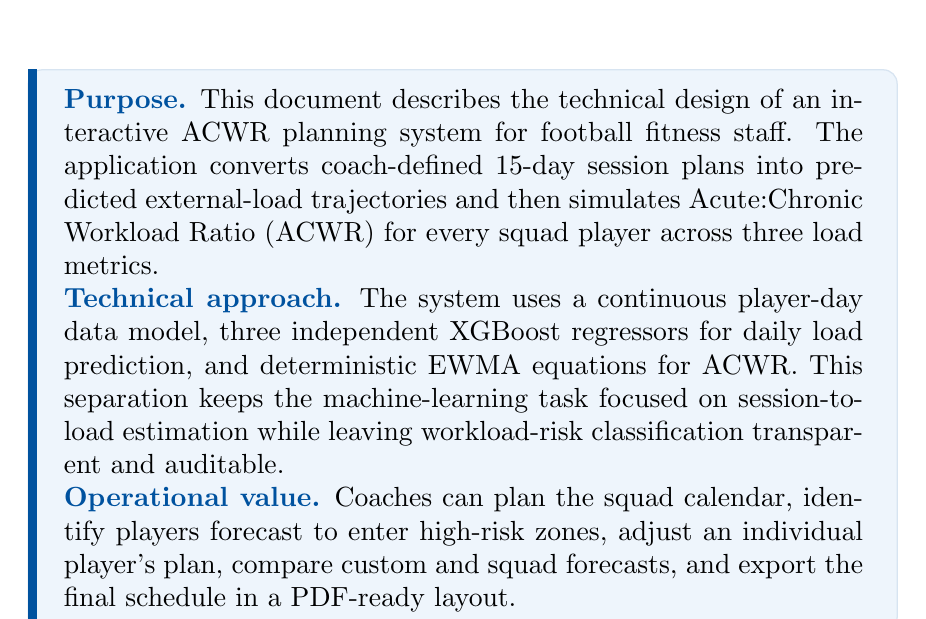
\begin{tikzpicture}
\node[
  draw=bordergray,
  fill=softblue,
  rounded corners=5pt,
  line width=0.45pt,
  inner sep=0pt
] (summarycard) {%
\begin{minipage}{0.91\textwidth}
\vspace{0.7em}
\hspace{0.95em}
\begin{minipage}{0.92\linewidth}
\textbf{\textcolor{rmblue}{Purpose.}} This document describes the technical design of an interactive ACWR planning system for football fitness staff. The application converts coach-defined 15-day session plans into predicted external-load trajectories and then simulates Acute:Chronic Workload Ratio (ACWR) for every squad player across three load metrics.

\textbf{\textcolor{rmblue}{Technical approach.}} The system uses a continuous player-day data model, three independent XGBoost regressors for daily load prediction, and deterministic EWMA equations for ACWR. This separation keeps the machine-learning task focused on session-to-load estimation while leaving workload-risk classification transparent and auditable.

\textbf{\textcolor{rmblue}{Operational value.}} Coaches can plan the squad calendar, identify players forecast to enter high-risk zones, adjust an individual player's plan, compare custom and squad forecasts, and export the final schedule in a PDF-ready layout.
\end{minipage}
\vspace{0.7em}
\end{minipage}};
\fill[rmblue] (summarycard.north west) rectangle ([xshift=0.12cm]summarycard.south west);
\end{tikzpicture}
\end{center}

\vspace{0.8em}
\begin{center}
\reportmetric{28}{squad players}
\hfill
\reportmetric{15}{forecast days}
\hfill
\reportmetric{3}{load metrics}
\hfill
\reportmetric{6,310}{player-days}
\end{center}

\vspace{0.8em}
\begin{table}[H]
\centering
\caption{Executive view of the solution.}
\begin{tabularx}{\textwidth}{L{3.5cm}Y}
\toprule
\rowcolor{softblue}
\tablehead{Dimension} & \tablehead{Summary} \\
\midrule
\textbf{Architecture} & Streamlit application backed by cached model bundles and a processed daily player grid. \\
\textbf{Data model} & Period-level GPS/session records are cleaned, capped, aggregated, and expanded into a continuous player-day calendar. \\
\textbf{Modeling} & One XGBoost model per target load metric; predictions are clipped to non-negative daily loads. \\
\textbf{ACWR method} & 7-day acute EWMA divided by 28-day chronic EWMA, with a 28-day warmup mask and explicit rest-day decay. \\
\textbf{User workflow} & Dashboard review, squad planning, forecast inspection, player-specific customization, and export. \\
\bottomrule
\end{tabularx}
\end{table}

\clearpage
\begingroup
\small
\setlength{\parskip}{0.15em}
\tableofcontents
\endgroup
\clearpage
\pagenumbering{arabic}
\pagestyle{fancy}

\section{Project Scope}

The application is an end-to-end decision-support tool for football workload planning. It does not predict injuries directly. Instead, it predicts future external training load from planned session types and converts those predicted loads into Acute:Chronic Workload Ratio (ACWR) trajectories.

The deployed application answers four operational questions:
\begin{enumerate}
  \item What is the current ACWR status of the squad across the three monitored load metrics?
  \item If coaches schedule a 15-day plan, which players are forecast to enter caution or danger zones?
  \item Can an individual player's plan be modified to reduce forecast risk while preserving the squad plan?
  \item Can the final squad plan be exported in a coach-readable PDF layout?
\end{enumerate}

\subsection{Core outputs}

\begin{itemize}
  \item Future daily load predictions for \code{total_distance}, \code{accelerations}, and \code{sprint_distance}.
  \item EWMA ACWR trajectories for each player and metric.
  \item Day-15 risk status and first date of danger-zone entry.
  \item A full-squad training schedule table with customized player plans marked.
\end{itemize}

\section{Solution Architecture}

The solution is split into three layers: a data/modeling package under \code{src/real_madrid_acwr}, a Streamlit application layer under \code{src/app}, and persisted artifacts under \code{data/processed} and \code{models/xgboost}.

\begin{figure}[H]
\centering
\resizebox{\textwidth}{!}{%
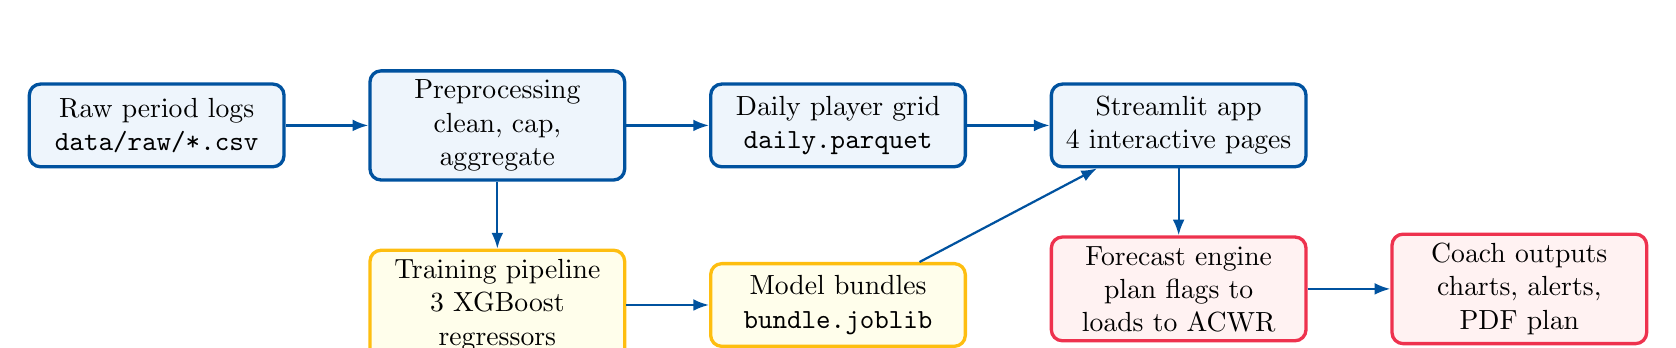
\begin{tikzpicture}[
  node distance=0.85cm and 1.05cm,
  box/.style={rectangle, rounded corners=4pt, draw=bordergray, fill=softgray, very thick, align=center, minimum width=3.0cm, minimum height=1.05cm, text width=3.0cm},
  bluebox/.style={box, draw=rmblue, fill=softblue},
  goldbox/.style={box, draw=rmgold, fill=yellow!8},
  redbox/.style={box, draw=rmred, fill=red!5},
  arrow/.style={-{Latex[length=2mm]}, thick, draw=rmblue}
]
\node[bluebox] (raw) {Raw period logs\\\code{data/raw/*.csv}};
\node[bluebox, right=of raw] (pipeline) {Preprocessing\\clean, cap, aggregate};
\node[bluebox, right=of pipeline] (daily) {Daily player grid\\\code{daily.parquet}};
\node[goldbox, below=of pipeline] (training) {Training pipeline\\3 XGBoost regressors};
\node[goldbox, right=of training] (bundles) {Model bundles\\\code{bundle.joblib}};
\node[bluebox, right=of daily] (app) {Streamlit app\\4 interactive pages};
\node[redbox, below=of app] (forecast) {Forecast engine\\plan flags to loads to ACWR};
\node[redbox, right=of forecast] (export) {Coach outputs\\charts, alerts, PDF plan};

\draw[arrow] (raw) -- (pipeline);
\draw[arrow] (pipeline) -- (daily);
\draw[arrow] (pipeline) -- (training);
\draw[arrow] (training) -- (bundles);
\draw[arrow] (daily) -- (app);
\draw[arrow] (bundles) -- (app);
\draw[arrow] (app) -- (forecast);
\draw[arrow] (forecast) -- (export);
\end{tikzpicture}
}
\caption{High-level system architecture. Production behavior is defined by the package under \code{src/}, the processed player-day table, and the model bundles.}
\label{fig:architecture}
\end{figure}

\subsection{Runtime components}

\begingroup
\small
\begin{longtable}{L{3.1cm}L{3.0cm}L{8.2cm}}
\caption{Runtime components and responsibilities. Component paths are shown relative to \code{src/}, except for \code{main.py}.}\\
\toprule
\rowcolor{softblue}
\tablehead{Component} & \tablehead{Layer} & \tablehead{Responsibility} \\
\midrule
\endfirsthead
\toprule
\rowcolor{softblue}
\tablehead{Component} & \tablehead{Layer} & \tablehead{Responsibility} \\
\midrule
\endhead
\componentcell{main.py}{entry point} & Streamlit shell & Dispatches the active page and injects app styling. \\
\addlinespace[0.25em]
\componentcell{app/pages.py}{UI rendering} & Application UI & Renders the Dashboard, Planning and Forecast, Player Customization, and Export Plan pages. \\
\addlinespace[0.25em]
\componentcell{app/planning.py}{calendar state} & Planning logic & Converts calendar events into the 15-day plan structure consumed by forecasting. \\
\addlinespace[0.25em]
\componentcell{app/forecasting.py}{inference flow} & Forecast engine & Builds inference frames, predicts future load, stitches forecast loads to history, and computes forecast ACWR. \\
\addlinespace[0.25em]
\componentcell{app/charts.py}{visualization} & Charting & Builds Plotly ACWR charts with historical and forecast load overlays. \\
\addlinespace[0.25em]
\componentcell{app/loaders.py}{cached resources} & Data access & Loads model bundles and \code{daily.parquet}; computes current player ACWR in cached Streamlit resources. \\
\addlinespace[0.25em]
\componentcell{acwr.py}{pure utility} & Core package & Computes EWMA ACWR and classifies risk zones. \\
\addlinespace[0.25em]
\componentcell{datapipeline.py}{preprocessing} & Modeling package & Applies shared cleaning, aggregation, feature engineering, and daily-spine construction. \\
\addlinespace[0.25em]
\componentcell{training/*.py}{model training} & Modeling package & Trains the three target-specific XGBoost regressors and writes deployable artifacts. \\
\addlinespace[0.25em]
\componentcell{artifacts.py}{serving contract} & Artifact loading & Validates and loads model bundles before serving. \\
\bottomrule
\end{longtable}
\endgroup

\section{Data Model}

\subsection{Raw source}

The bootstrap archive is \code{data/raw/data_acute_vs_chronic.zip}; when needed, the pipeline extracts it to \code{data/raw/data_acute_vs_chronic.csv}. The raw table contains one row per training period or drill block, not one row per player-day.

\begin{table}[H]
\centering
\caption{Important raw fields and deployed interpretations.}
\begin{tabularx}{\textwidth}{L{4.65cm}Y}
\toprule
\rowcolor{softblue}
\tablehead{Field} & \tablehead{Interpretation} \\
\midrule
\textbf{\code{player_id}} & Player identifier used throughout the application. \\
\textbf{\code{position_name_en}} & Position label displayed in tables and player selectors. \\
\textbf{\code{height}}, \textbf{\code{weight}}, \textbf{\code{date_of_birth}} & Player profile features. Age is computed during cleaning and rounded to whole years by the current pipeline. \\
\textbf{\code{period_start_time}} & Period timestamp, normalized to a calendar date. \\
\textbf{\code{period_name}} & Session family prefix. Examples: \code{G 1960}, \code{TAC 0133}, \code{BP 2351}. Missing values are mapped to \code{MATCH}. \\
\textbf{\code{activity_id}} & Used to count period rows per player-day. \\
\textbf{\code{total_distance}} & Daily total-distance target after aggregation. \\
\begin{tabular}[t]{@{}l@{}}\code{acc_band7plus_total_}\\\code{effort_count}\end{tabular} & Renamed to \code{accelerations}. \\
\begin{tabular}[t]{@{}l@{}}\code{velocity_band6plus7_}\\\code{total_distance}\end{tabular} & Renamed to \code{sprint_distance}. \\
\bottomrule
\end{tabularx}
\end{table}

\subsection{Session taxonomy}

\begin{table}[H]
\centering
\caption{Session families used in planning, modeling, and export.}
\begin{tabular}{L{2.5cm}L{8.5cm}}
\toprule
\rowcolor{softblue}
\tablehead{Code} & \tablehead{Meaning} \\
\midrule
\textbf{G} & Game-based work / small-sided games. \\
\textbf{TAC} & Tactical training. \\
\textbf{BP} & Set pieces. \\
\textbf{TEC} & Technical training. \\
\textbf{MATCH} & Official match. \\
\textbf{REST} & No planned session. Encoded as zero load and zero session flags. \\
\bottomrule
\end{tabular}
\end{table}

\subsection{Processed daily table}

The primary serving dataset is \code{data/processed/daily.parquet}. It contains a complete daily calendar spine for each retained player, with rest days inserted as explicit zero-load rows.

\begin{table}[H]
\centering
\caption{Current processed data contract.}
\begin{tabular}{L{4.4cm}L{8.0cm}}
\toprule
\rowcolor{softblue}
\tablehead{Property} & \tablehead{Value} \\
\midrule
\textbf{Rows} & 6,310 player-days \\
\textbf{Players} & 28 \\
\textbf{Date range} & 2024-07-16 to 2025-06-26 \\
\textbf{Granularity} & One row per \code{player_id} and calendar \code{date} \\
\textbf{Load targets} & \code{total_distance}, \code{accelerations}, \code{sprint_distance} \\
\textbf{Session flags} & \code{has_BP}, \code{has_G}, \code{has_MATCH}, \code{has_TAC}, \code{has_TEC} \\
\textbf{Activity fields} & \code{n_periods}, \code{n_exercise_types} \\
\textbf{Profile fields} & \code{height}, \code{weight}, \code{age}, \code{position} \\
\bottomrule
\end{tabular}
\end{table}

\begin{figure}[H]
\centering
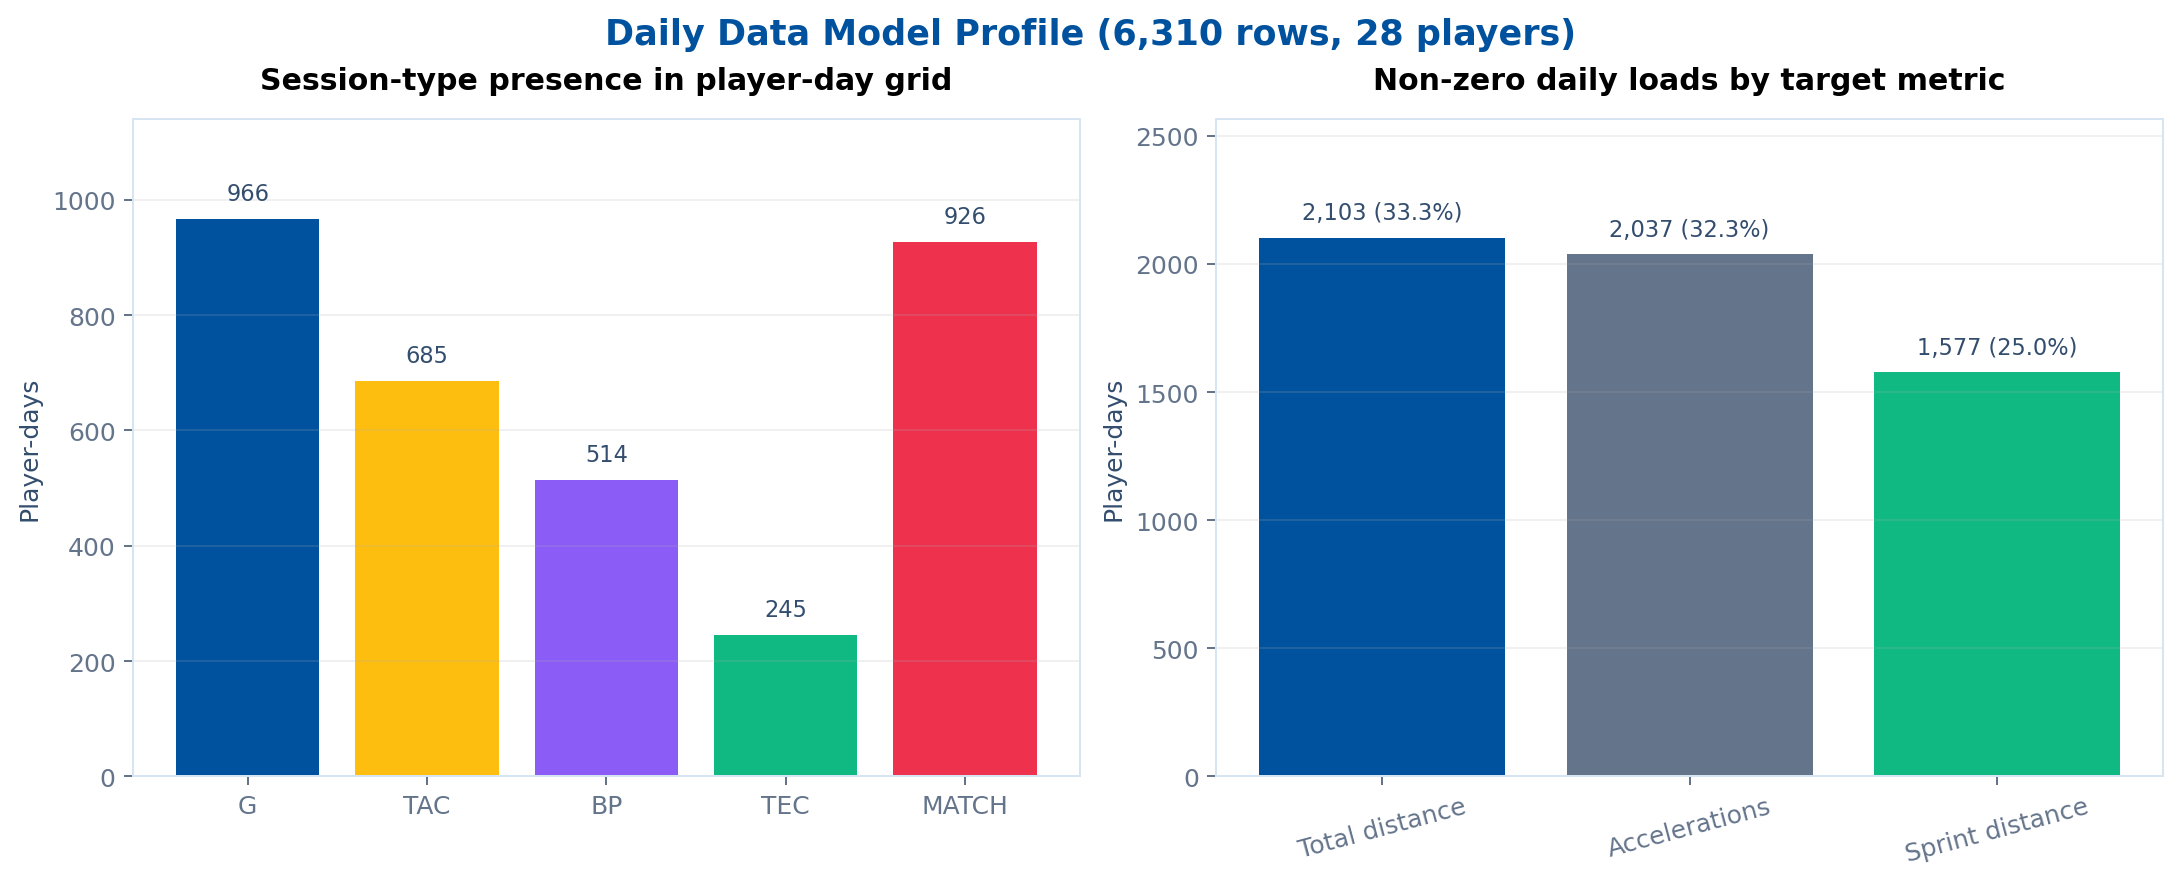
\includegraphics[width=\textwidth]{generated/daily_data_profile.png}
\caption{Profile of the processed player-day grid. The left panel shows how often each session flag appears. The right panel shows the number and share of player-days with non-zero load by target metric.}
\label{fig:daily-profile}
\end{figure}

\subsection{Inference plan frame}

At forecast time, the calendar plan is converted into one row per player and forecast day. For a 15-day horizon and 28 players, each target model receives 420 rows. Each row contains the planned session flags, activity counts, player profile fields, and day-of-week one-hot features.

\begin{figure}[H]
\centering
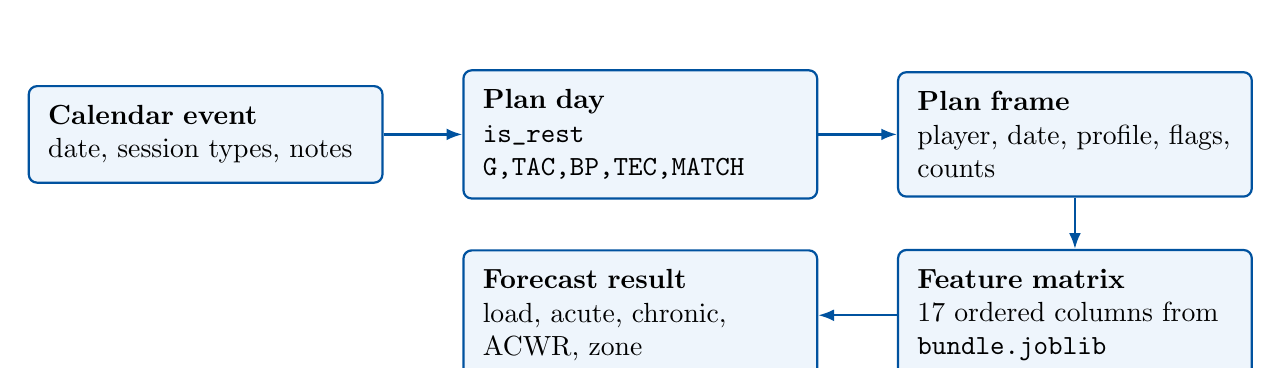
\begin{tikzpicture}[
  node distance=0.65cm and 1.0cm,
  entity/.style={rectangle, rounded corners=3pt, draw=rmblue, fill=softblue, thick, align=left, text width=4.0cm, inner sep=7pt},
  arrow/.style={-{Latex[length=2mm]}, thick, draw=rmblue}
]
\node[entity] (calendar) {\textbf{Calendar event}\\date, session types, notes};
\node[entity, right=of calendar] (plandays) {\textbf{Plan day}\\\code{is_rest}\\\code{G,TAC,BP,TEC,MATCH}};
\node[entity, right=of plandays] (planframe) {\textbf{Plan frame}\\player, date, profile, flags, counts};
\node[entity, below=of planframe] (features) {\textbf{Feature matrix}\\17 ordered columns from \code{bundle.joblib}};
\node[entity, left=of features] (outputs) {\textbf{Forecast result}\\load, acute, chronic, ACWR, zone};
\draw[arrow] (calendar) -- (plandays);
\draw[arrow] (plandays) -- (planframe);
\draw[arrow] (planframe) -- (features);
\draw[arrow] (features) -- (outputs);
\end{tikzpicture}
\caption{Forecast data flow from calendar events to the final result object.}
\label{fig:data-contracts}
\end{figure}

\section{Methodology}

\subsection{Cleaning and cohort definition}

The preprocessing pipeline applies the following steps:
\begin{enumerate}
  \item Rename raw load columns to the deployed metric names.
  \item Normalize timestamps and derive \code{exercise_type} from the session prefix.
  \item Fill missing match flags, then drop the raw match flag after deriving session type.
  \item Compute age from date of birth and session date; the current pipeline rounds age to whole years.
  \item Drop rows with missing player metadata.
  \item Apply IQR capping at \(Q_3 + 3 \times IQR\) per player and exercise type for \code{total_distance}, and also for the target metric when training \code{accelerations} or \code{sprint_distance}.
  \item Drop players with placeholder \code{weight == 200}.
  \item Aggregate period rows into player-day rows.
  \item Build a complete daily spine per player and fill rest days with zero load.
\end{enumerate}

Rest-day filling is not cosmetic. ACWR is a daily time-series calculation, so missing calendar days must decay the acute and chronic EWMA states with zero load rather than disappear from the sequence.

\subsection{Feature engineering}

The deployed feature set is cross-sectional: all features are known before the planned day starts. The model does not receive lagged load, previous ACWR, player identifiers, or injury labels.

\begin{table}[H]
\centering
\caption{Feature groups persisted in each deployed model bundle.}
\begin{tabularx}{\textwidth}{L{3.7cm}Y}
\toprule
\rowcolor{softblue}
\tablehead{Group} & \tablehead{Features} \\
\midrule
\textbf{Activity volume} & \code{n_periods}, \code{n_exercise_types} \\
\textbf{Session family} & \code{has_BP}, \code{has_G}, \code{has_MATCH}, \code{has_TAC}, \code{has_TEC} \\
\textbf{Player profile} & \code{height}, \code{weight}, \code{age} \\
\textbf{Calendar} & \code{dow_0}, \code{dow_1}, \code{dow_2}, \code{dow_3}, \code{dow_4}, \code{dow_5}, \code{dow_6} \\
\bottomrule
\end{tabularx}
\end{table}

The currently saved \code{bundle.joblib} artifacts each contain 17 ordered feature columns. The serving code always uses the feature order stored in the bundle, so training and inference stay aligned even if the column order in a DataFrame changes.

\subsection{Model training}

The system trains three independent XGBoost regressors: one for total distance, one for accelerations, and one for sprint distance. Each model is trained on a \(\log(1+y)\)-transformed target, with a \code{MinMaxScaler} fit on the training features only.

\begin{align}
\tilde{y} &= \log(1 + y) \\
\hat{y} &= \max(\exp(\hat{\tilde{y}}) - 1, 0)
\end{align}

The training scripts use:
\begin{itemize}
  \item random 80/20 train/test split with \code{random_state=42};
  \item 10-fold shuffled \code{KFold} cross-validation;
  \item \code{RandomizedSearchCV} with 50 sampled configurations;
  \item \code{XGBRegressor(objective="reg:squarederror", tree_method="hist")}.
\end{itemize}

\begin{table}[H]
\centering
\caption{Evaluation of the saved bundles on the deterministic held-out split.}
\begin{tabular}{L{3.3cm}L{2.1cm}r r r r}
\toprule
\rowcolor{softblue}
\tablehead{Target} & \tablehead{Unit} & \tablehead{Features} & \tablehead{RMSE} & \tablehead{MAE} & \tablehead{\(R^2\)} \\
\midrule
\textbf{\code{total_distance}} & metres & 17 & 569.98 & 223.64 & 0.831 \\
\textbf{\code{accelerations}} & count & 17 & 2.73 & 1.09 & 0.750 \\
\textbf{\code{sprint_distance}} & metres & 17 & 15.02 & 5.38 & 0.352 \\
\bottomrule
\end{tabular}
\end{table}

\begin{figure}[H]
\centering
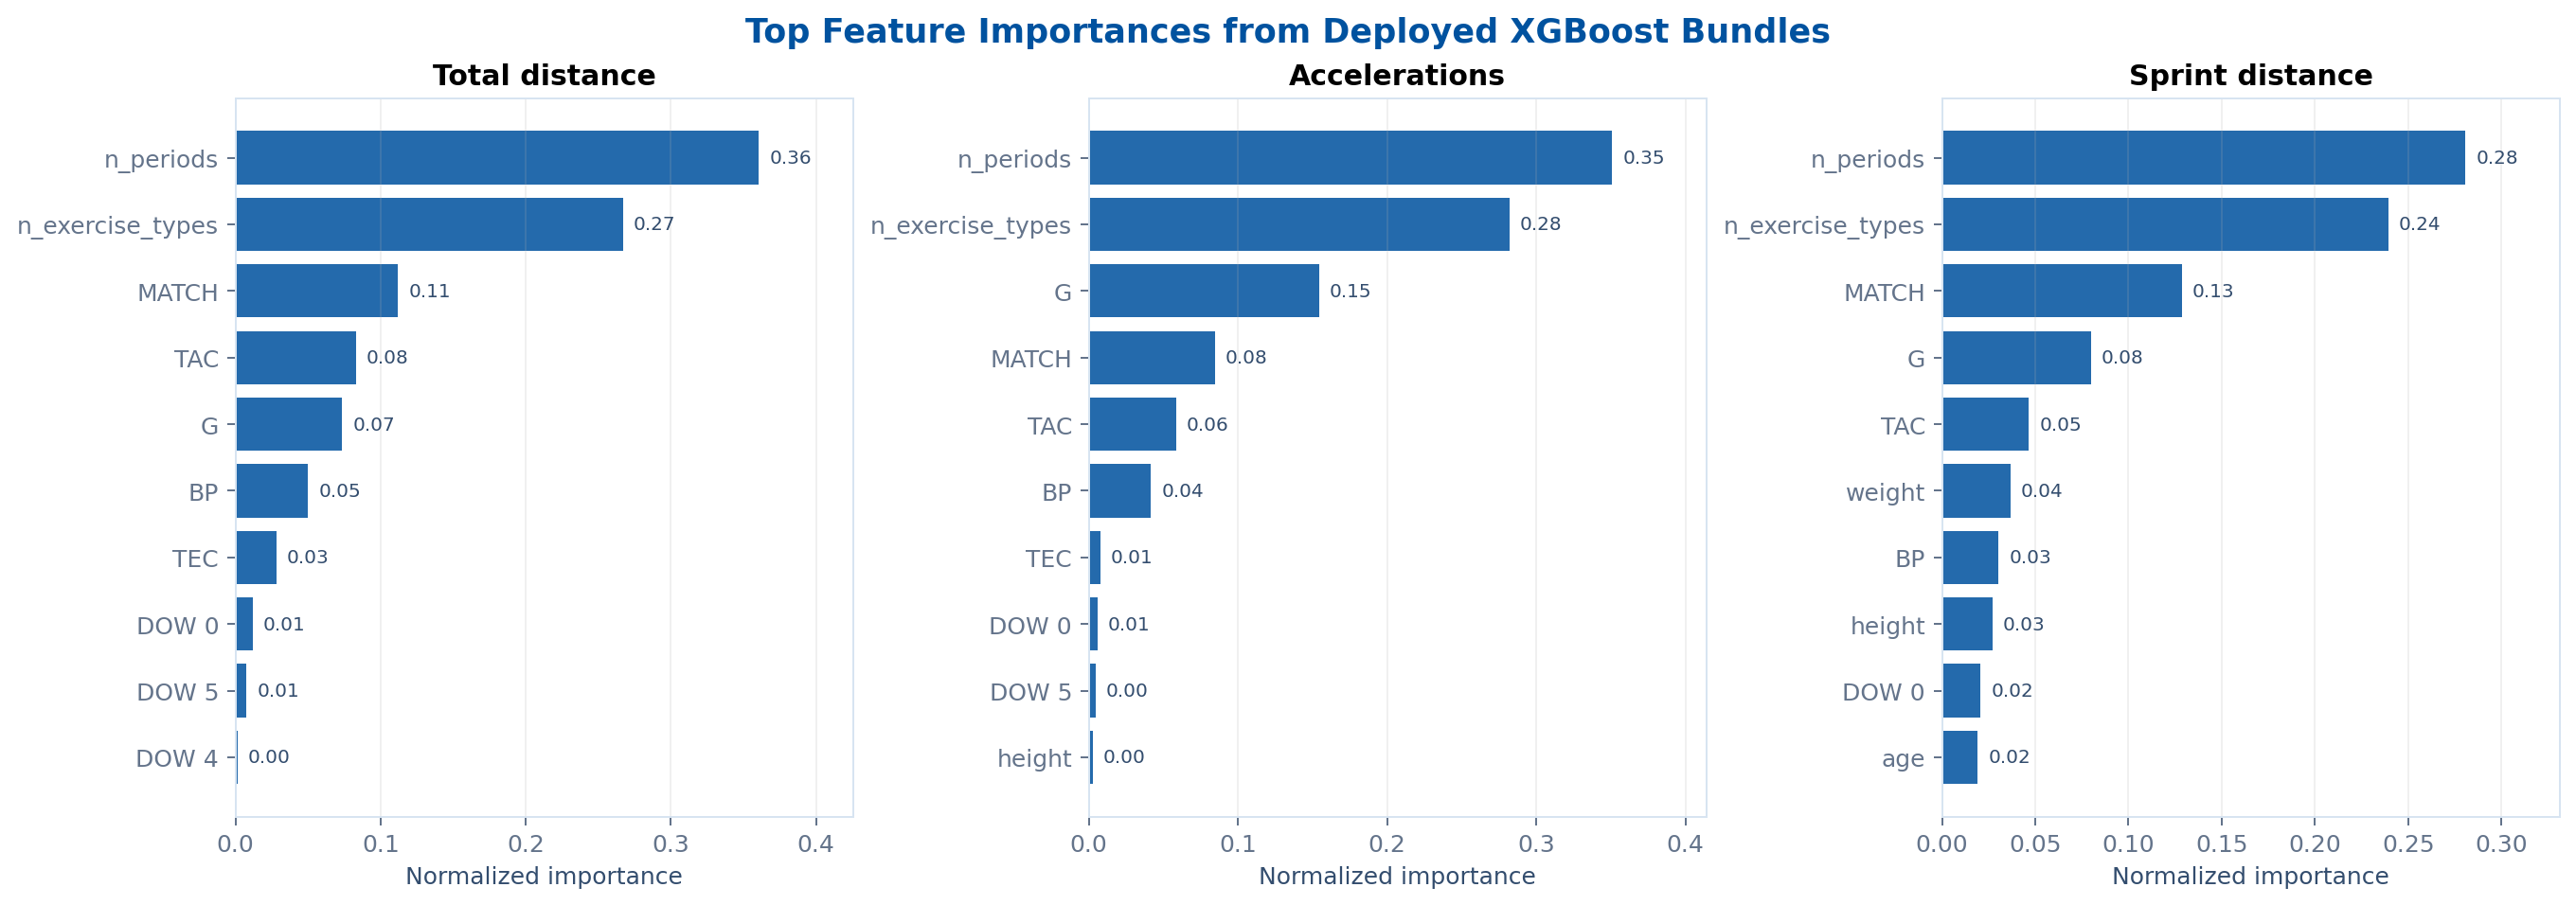
\includegraphics[width=\textwidth]{generated/model_feature_importance.png}
\caption{Top feature importances from the three deployed XGBoost bundles. Activity counts and session-family flags dominate the serving models.}
\label{fig:model-importance}
\end{figure}

\subsection{Model and report figures}

The repository also contains generated report figures under \code{reports/figures}. These are included here as model-development evidence and exploratory context.

\begin{figure}[H]
\centering
\begin{subfigure}{0.32\textwidth}
  \centering
  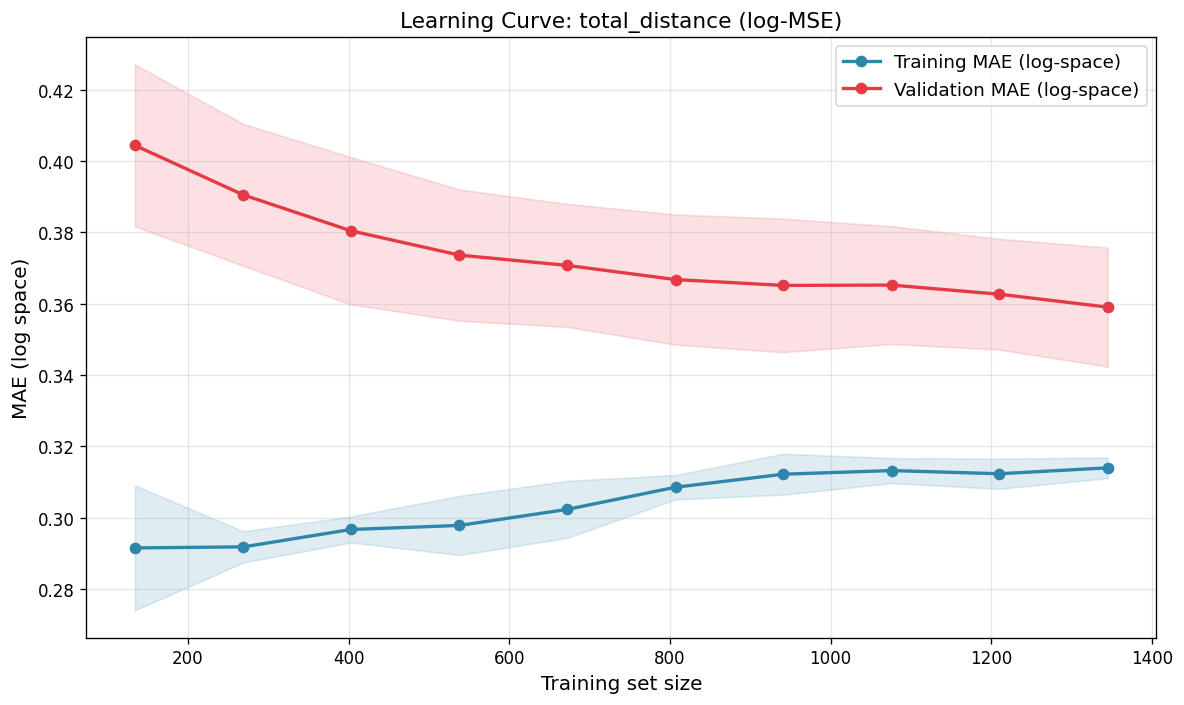
\includegraphics[width=\linewidth]{reports/total_distance_learning_curve.png}
  \caption{Total distance}
\end{subfigure}
\hfill
\begin{subfigure}{0.32\textwidth}
  \centering
  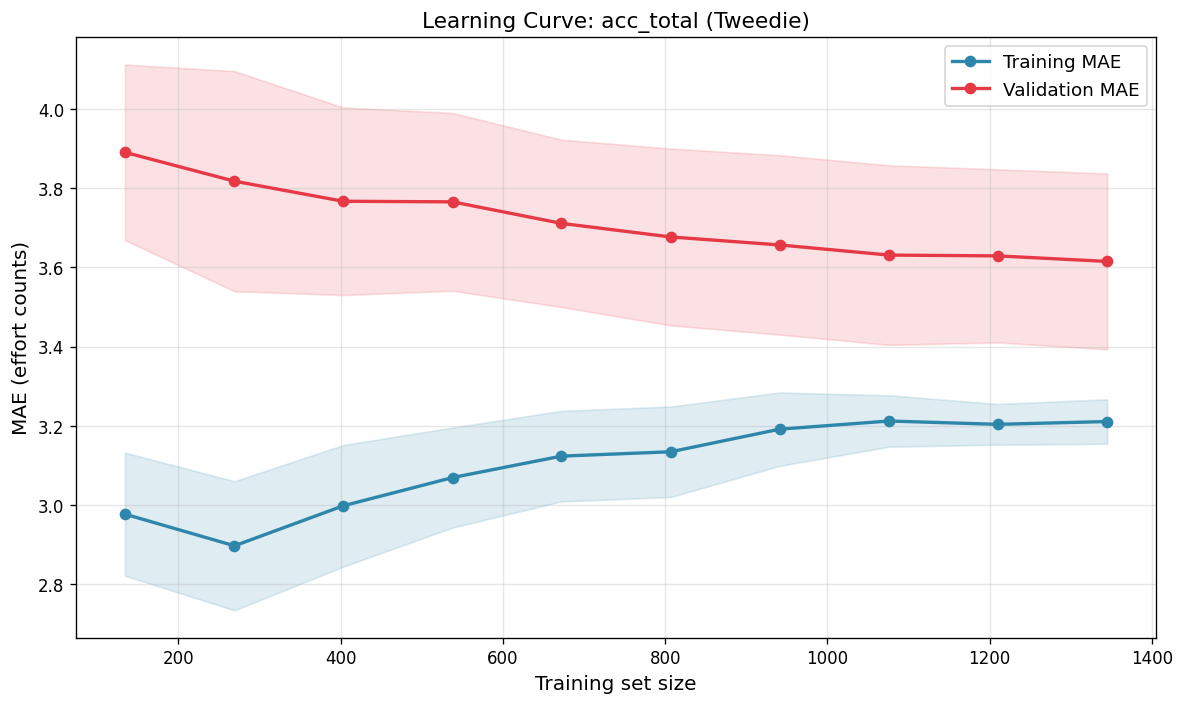
\includegraphics[width=\linewidth]{reports/accelerations_learning_curve.png}
  \caption{Accelerations}
\end{subfigure}
\hfill
\begin{subfigure}{0.32\textwidth}
  \centering
  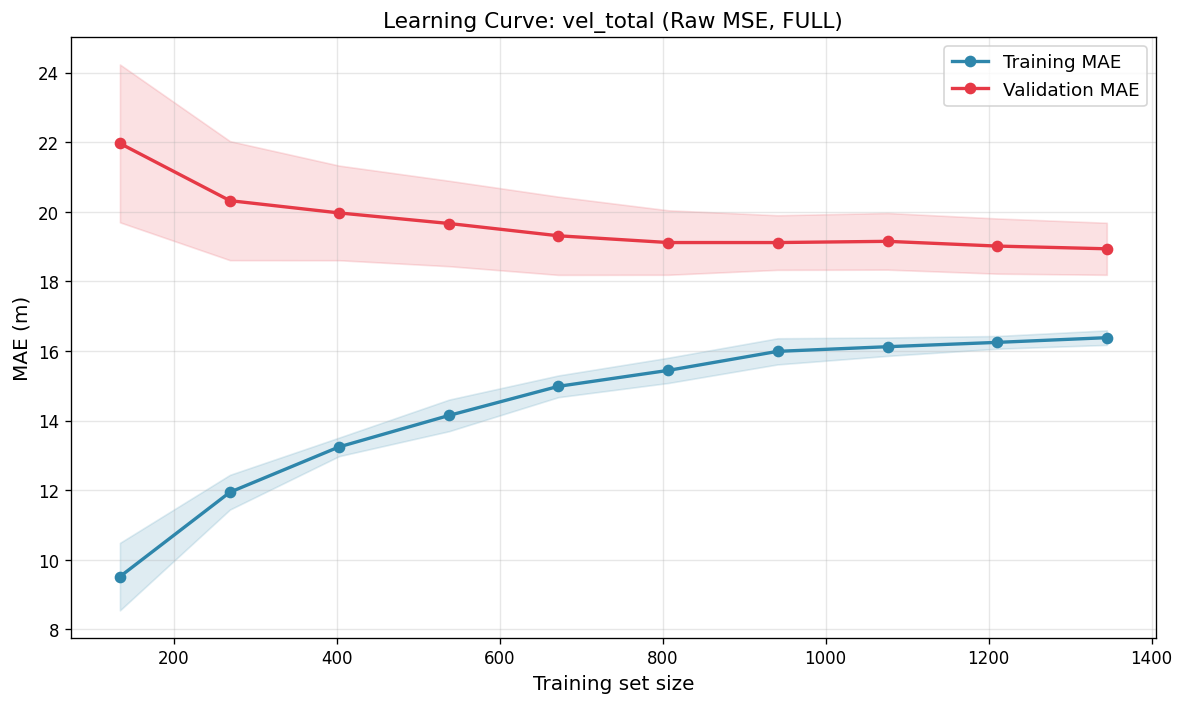
\includegraphics[width=\linewidth]{reports/sprint_distance_learning_curve.png}
  \caption{Sprint distance}
\end{subfigure}
\caption{Learning-curve figures copied from the model reports.}
\label{fig:learning-curves}
\end{figure}

\begin{figure}[H]
\centering
\begin{subfigure}{0.48\textwidth}
  \centering
  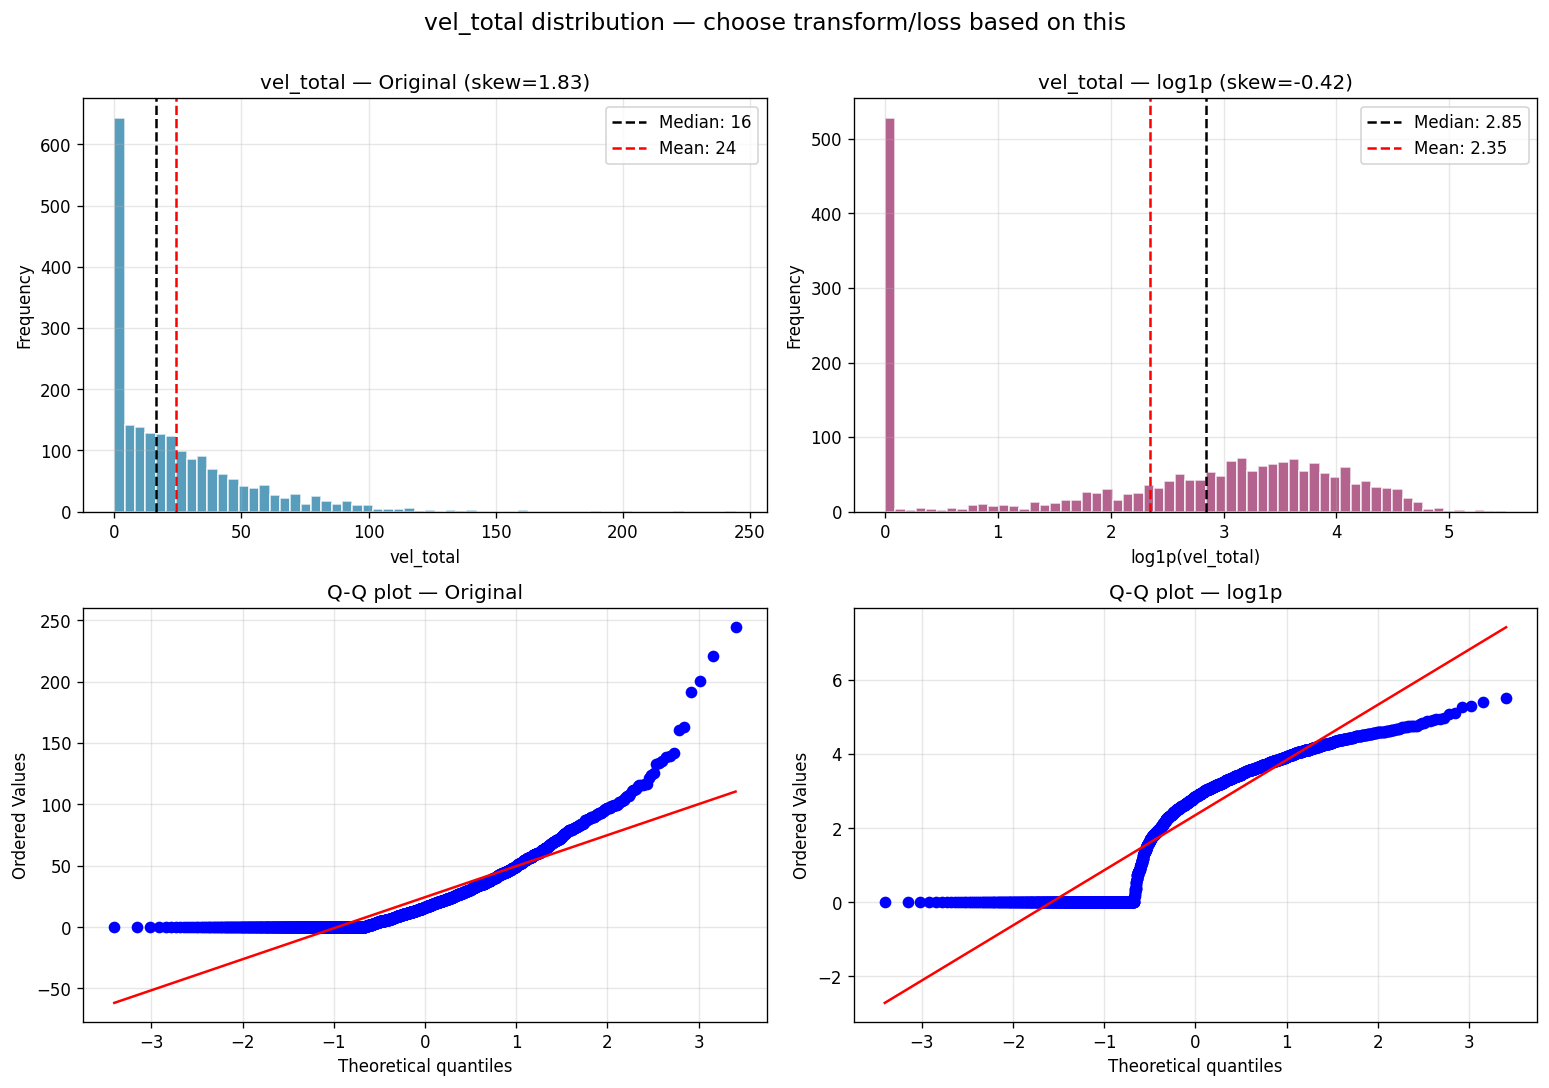
\includegraphics[width=\linewidth]{reports/sprint_distance_distribution.png}
  \caption{Sprint-distance distribution}
\end{subfigure}
\hfill
\begin{subfigure}{0.48\textwidth}
  \centering
  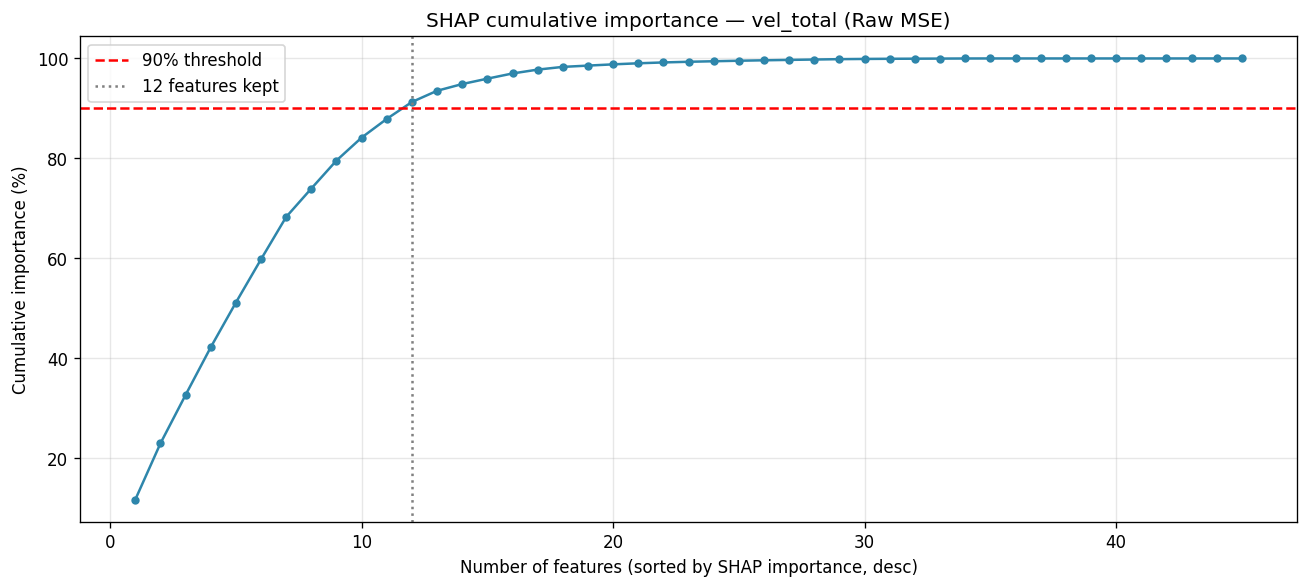
\includegraphics[width=\linewidth]{reports/sprint_distance_shap_cumulative.png}
  \caption{Cumulative SHAP context}
\end{subfigure}
\caption{Additional report figures for the high-speed running target.}
\label{fig:report-sprint}
\end{figure}

\subsection{ACWR computation}

ACWR is computed after load prediction. The models forecast load; the sport-science ratio is a deterministic transformation of historical and forecast daily load.

For a daily load series \(L_t\), the system computes uncoupled exponentially weighted moving averages:

\begin{align}
\text{acute}_t &= \alpha_a L_t + (1-\alpha_a)\text{acute}_{t-1},
& \alpha_a &= \frac{2}{7+1} = 0.25 \\
\text{chronic}_t &= \alpha_c L_t + (1-\alpha_c)\text{chronic}_{t-1},
& \alpha_c &= \frac{2}{28+1} \approx 0.069
\end{align}

\[
\text{ACWR}_t = \frac{\text{acute}_t}{\text{chronic}_t}
\]

The first 28 rows of each player's history are masked because the chronic EWMA has not stabilized. If chronic load is zero, ACWR is reported as unavailable.

\begin{table}[H]
\centering
\caption{Operational ACWR risk zones used by the application.}
\begin{tabular}{L{3.0cm}L{3.0cm}L{7.2cm}}
\toprule
\rowcolor{softblue}
\tablehead{Zone} & \tablehead{ACWR range} & \tablehead{Interpretation} \\
\midrule
\riskbadge{rmgray}{Under} & \(<0.8\) & Insufficient load stimulus or recent unloading. \\
\riskbadge{rmgreen}{Optimal} & \(0.8 \leq ACWR < 1.3\) & Target training range. \\
\riskbadge{rmgold}{Caution} & \(1.3 \leq ACWR < 1.5\) & Elevated workload signal; monitor closely. \\
\riskbadge{rmred}{Danger} & \(\geq 1.5\) & High workload spike signal; consider reducing load. \\
\bottomrule
\end{tabular}
\end{table}

\subsection{Forecast algorithm}

The forecast engine is direct and non-recursive:
\begin{enumerate}
  \item Convert calendar events into 15 plan-day dictionaries.
  \item Build a plan frame with one row per player and day.
  \item Add day-of-week one-hot columns.
  \item Align the matrix to \code{feature_cols} from each \code{bundle.joblib}.
  \item Predict all plan rows for a target in one XGBoost call.
  \item Force rest-day predictions to zero where \code{n_periods == 0}.
  \item Append the 15 predicted loads to the player's historical daily loads.
  \item Recompute EWMA ACWR on the stitched history-plus-forecast series.
  \item Extract forecast curves, day-15 ACWR, and risk zones.
\end{enumerate}

This separation keeps the model interpretable: the regressor estimates daily external load from the planned session composition, while the ACWR module simulates how that load path changes short-term versus long-term workload state.

\section{Interactive App User Guide}

Run the app from the project root:

\begin{verbatim}
python -m pip install -e ".[dev]"
streamlit run main.py
\end{verbatim}

The sidebar contains the page navigation and ENG/ESP language toggle. The application has four pages.

\subsection{Dashboard}

The Dashboard summarizes the current state of the squad using the latest available historical data. It explains the ACWR formula, shows the EWMA smoothing setup, defines risk zones, and lists each player with current ACWR values for the three load metrics.

Recommended use:
\begin{enumerate}
  \item Review high-risk and caution counts before planning the next cycle.
  \item Check whether risk is isolated to one metric or appears across multiple metrics.
  \item Treat the values as workload signals, not medical diagnoses.
\end{enumerate}

\subsection{Planning and Forecast}

The Planning and Forecast page is the main workflow for squad planning. Coaches create calendar events inside the 15-day forecast window, assign one or more session types, and run the forecast.

\begin{figure}[H]
\centering
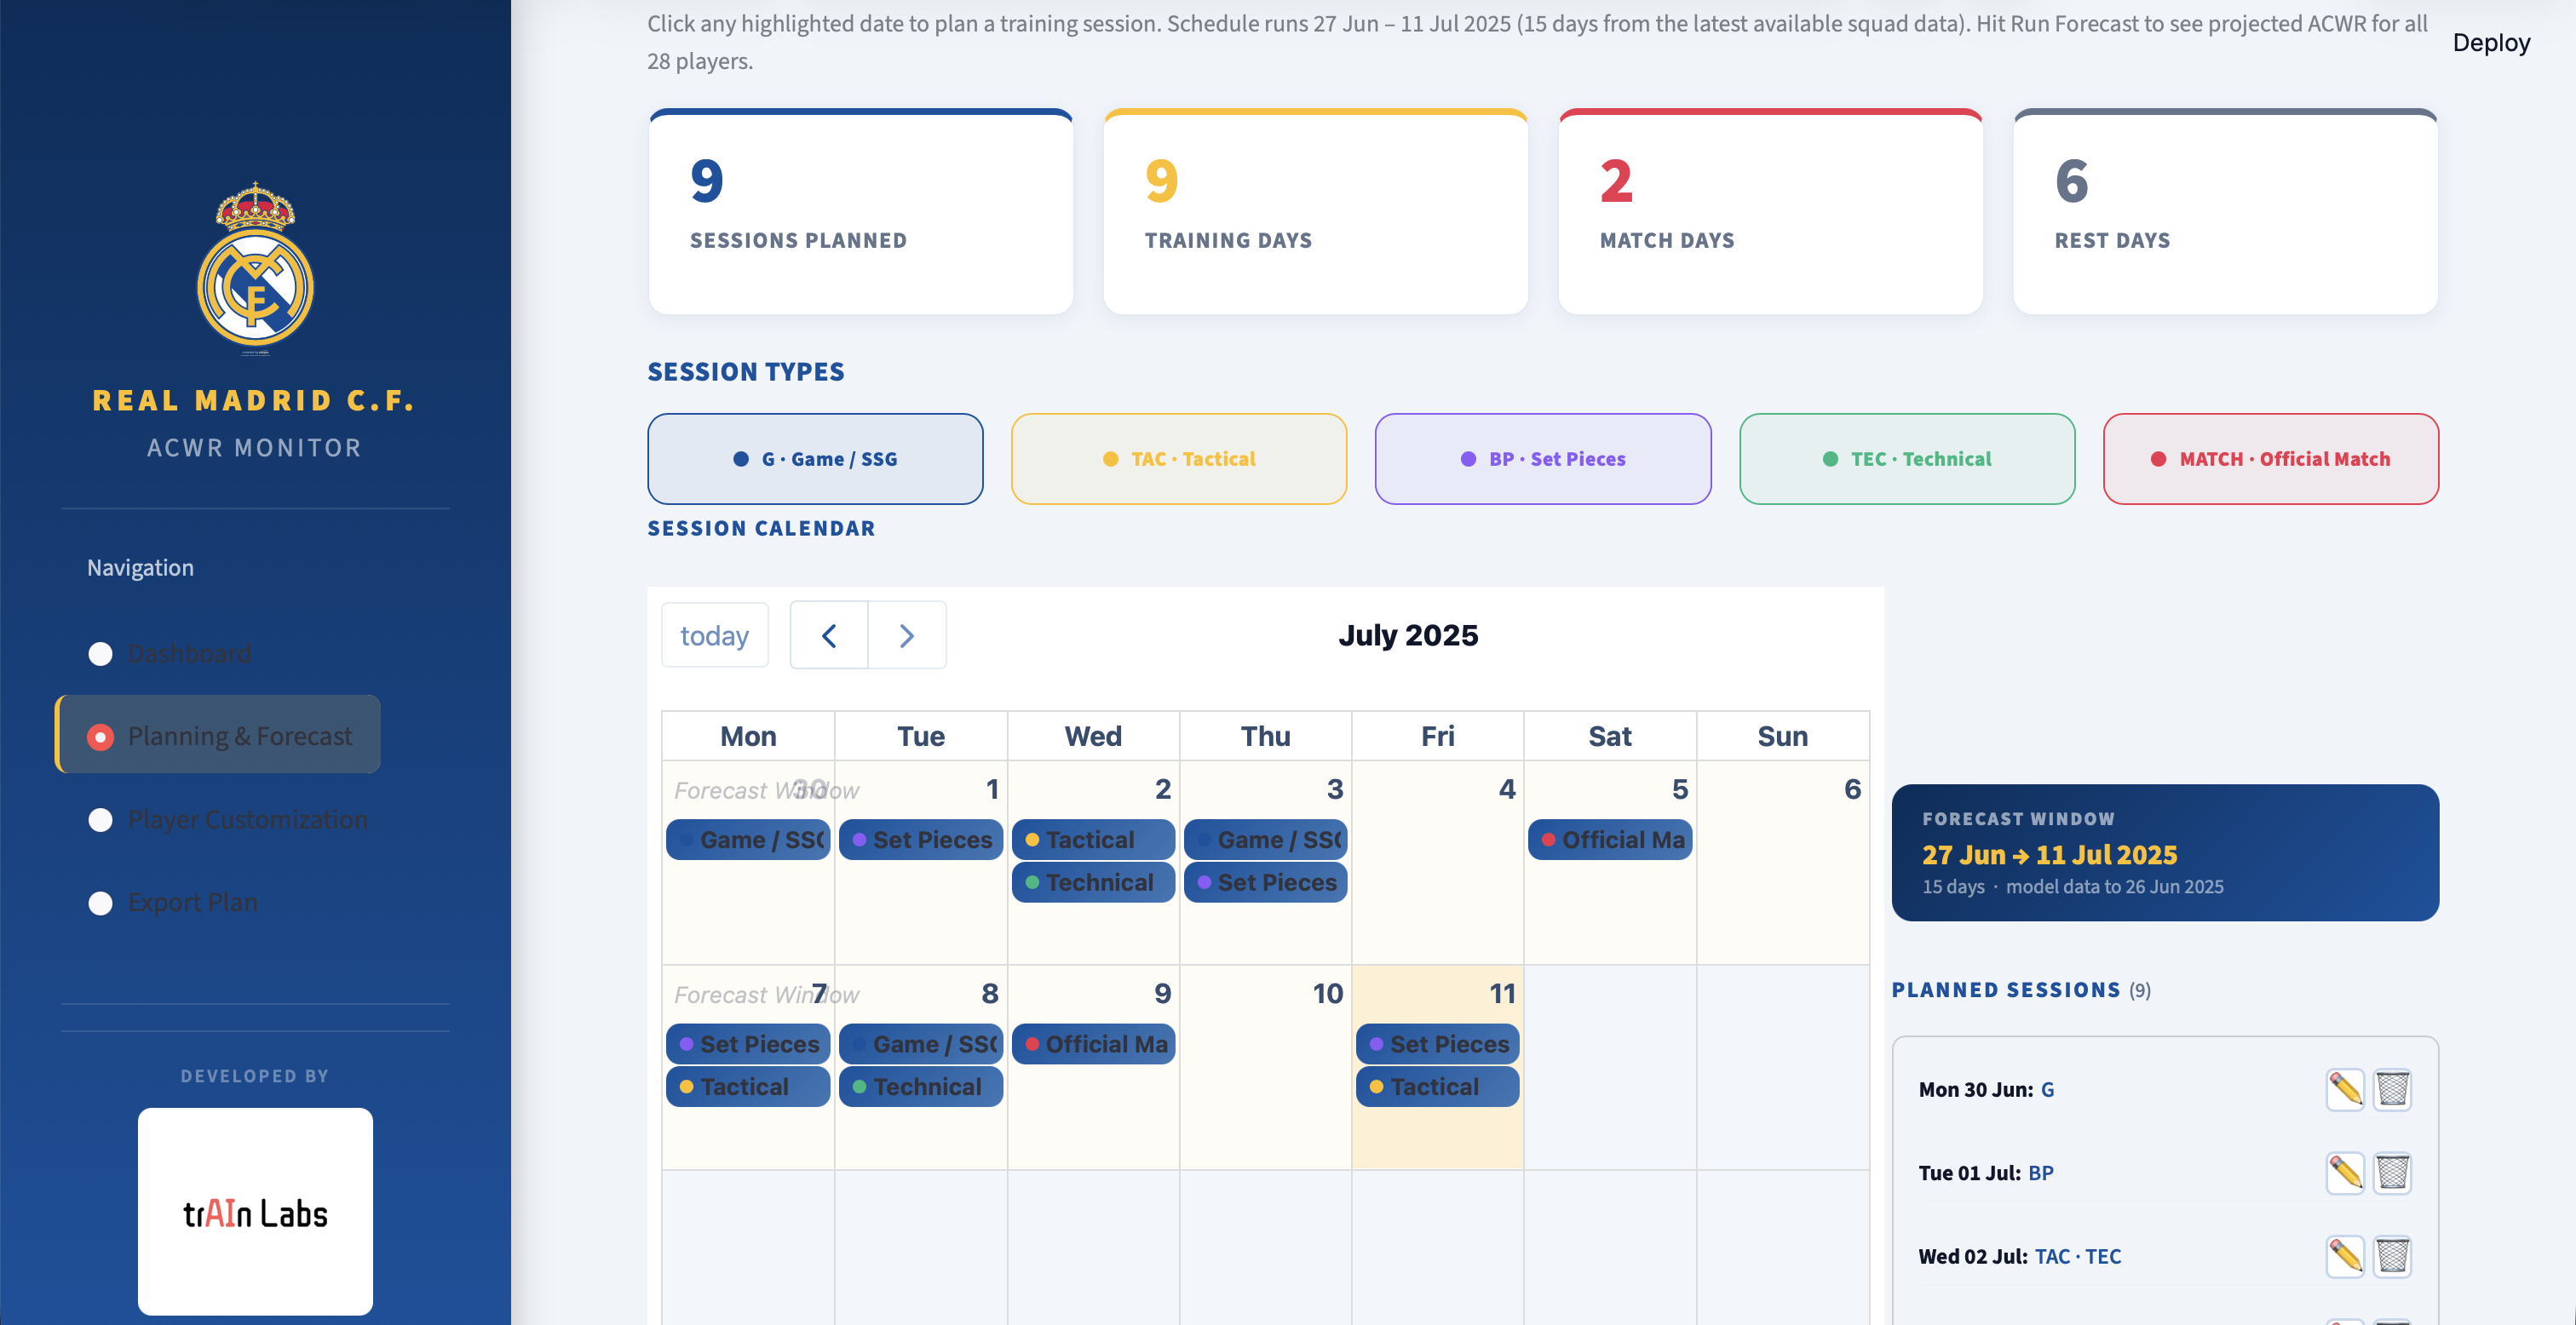
\includegraphics[width=\textwidth]{screenshots/planning_calendar.png}
\caption{Planning page with FullCalendar event creation, plan KPIs, session-type legend, and the planned-session list.}
\label{fig:planning-calendar}
\end{figure}

Workflow:
\begin{enumerate}
  \item Click a highlighted date in the forecast window.
  \item Select session types: G, TAC, BP, TEC, or MATCH.
  \item Save the event. Multiple session types can be scheduled on the same day.
  \item Repeat until the 15-day plan is complete.
  \item Click \textbf{Run Forecast}.
\end{enumerate}

After forecasting, the app shows an injury-risk alert if any player enters the danger zone during the forecast horizon.

\begin{figure}[H]
\centering
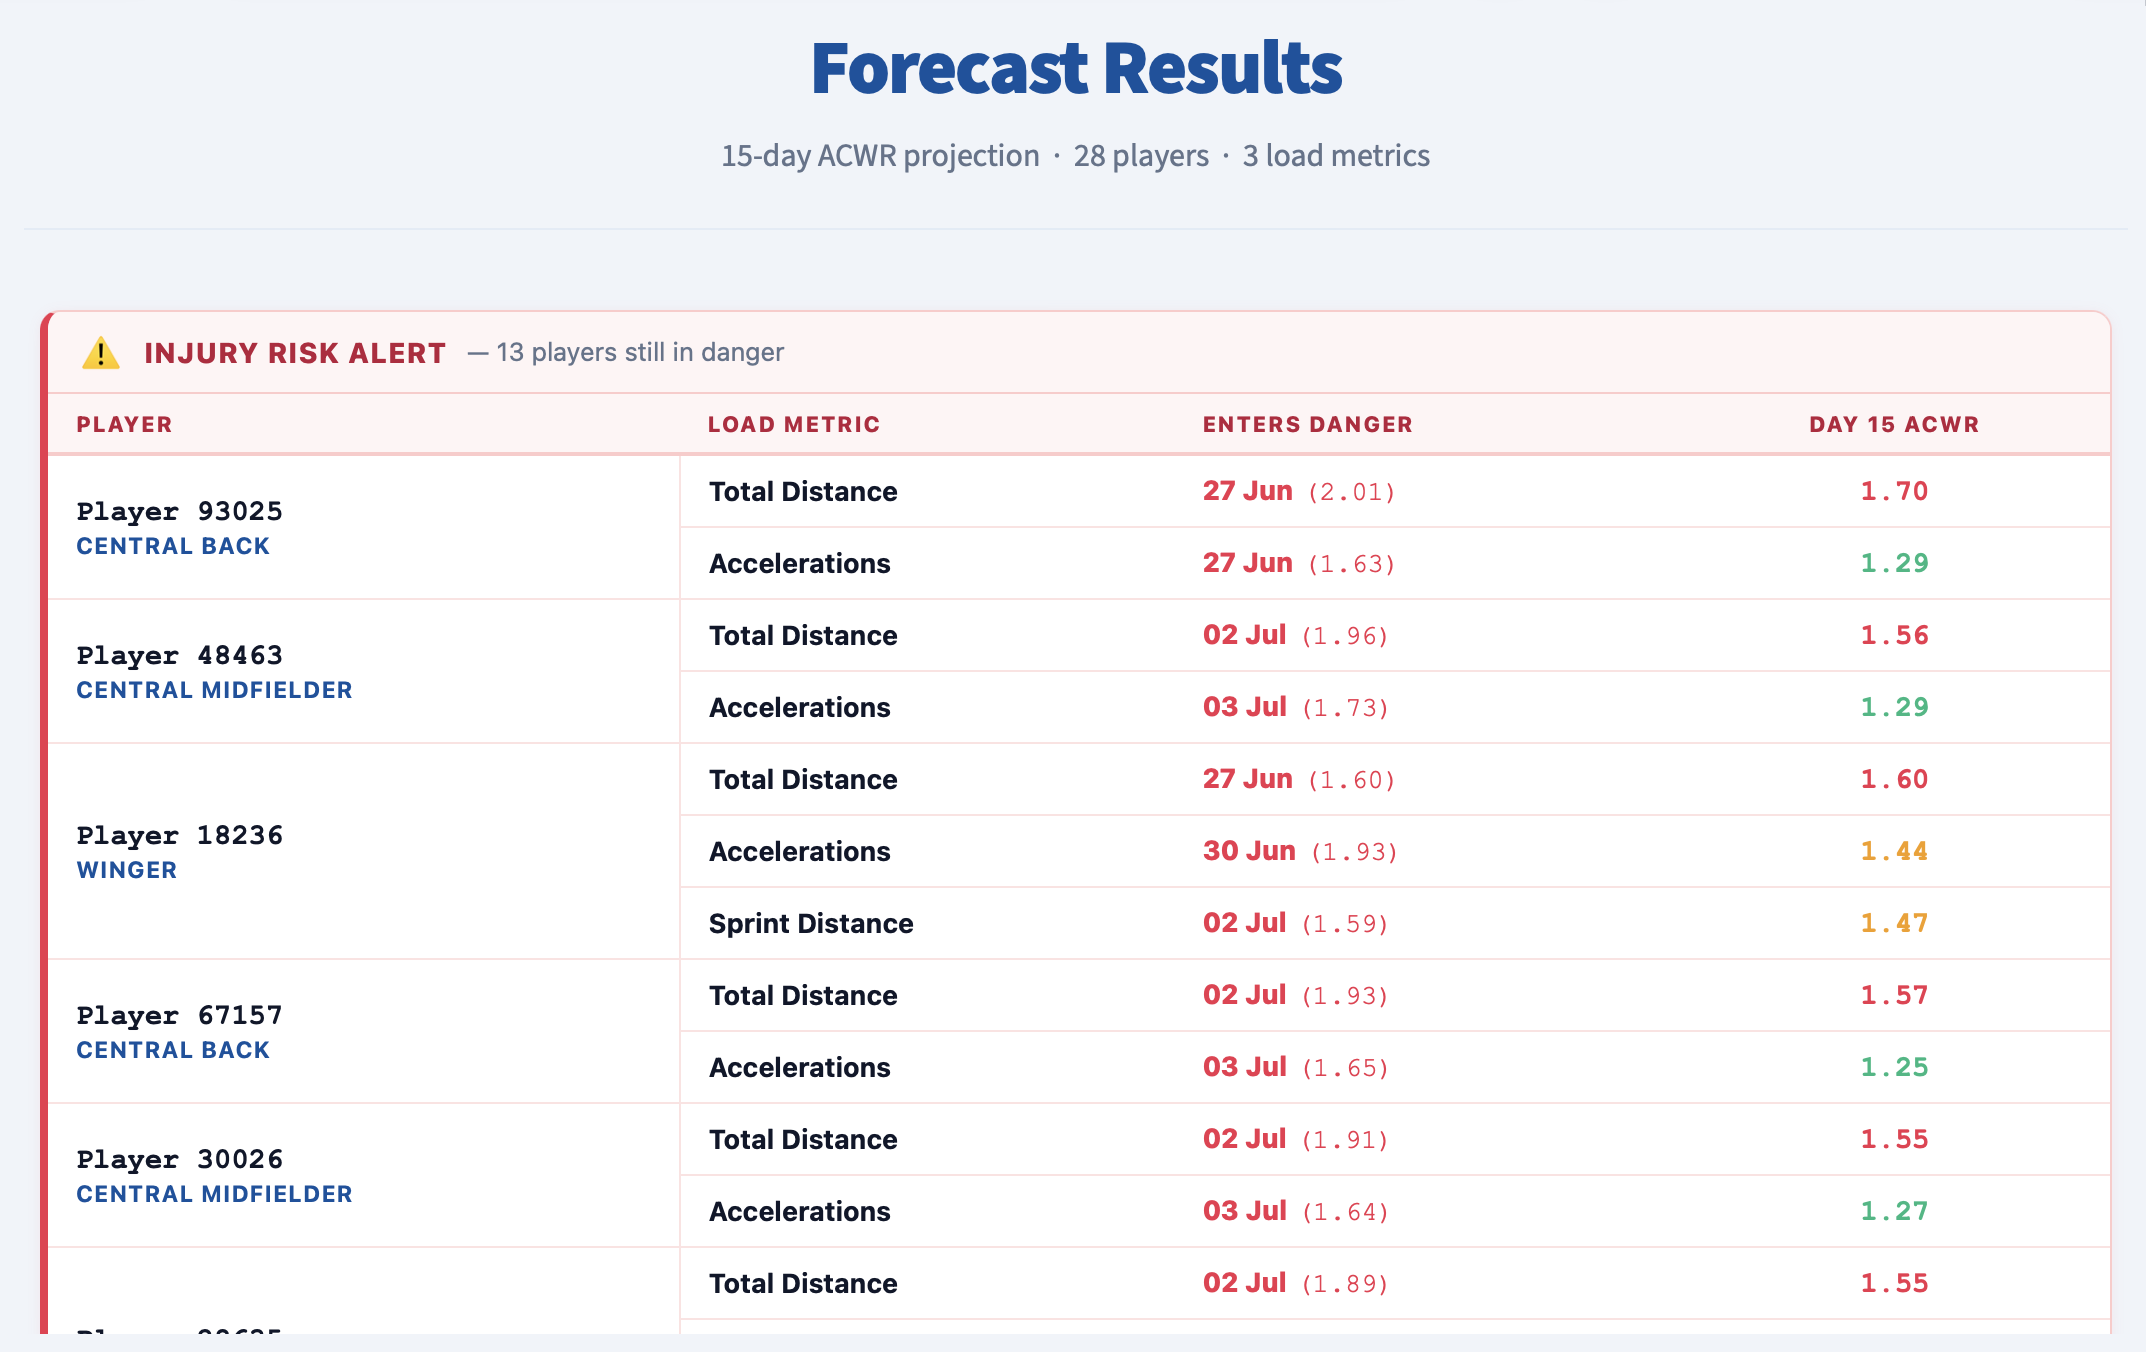
\includegraphics[width=\textwidth]{screenshots/forecast_alert.png}
\caption{Forecast alert table listing players and metrics that enter the danger zone.}
\label{fig:forecast-alert}
\end{figure}

For a selected player, the page renders one chart per metric. The chart can optionally show load bars beneath the ACWR line.

\begin{figure}[H]
\centering
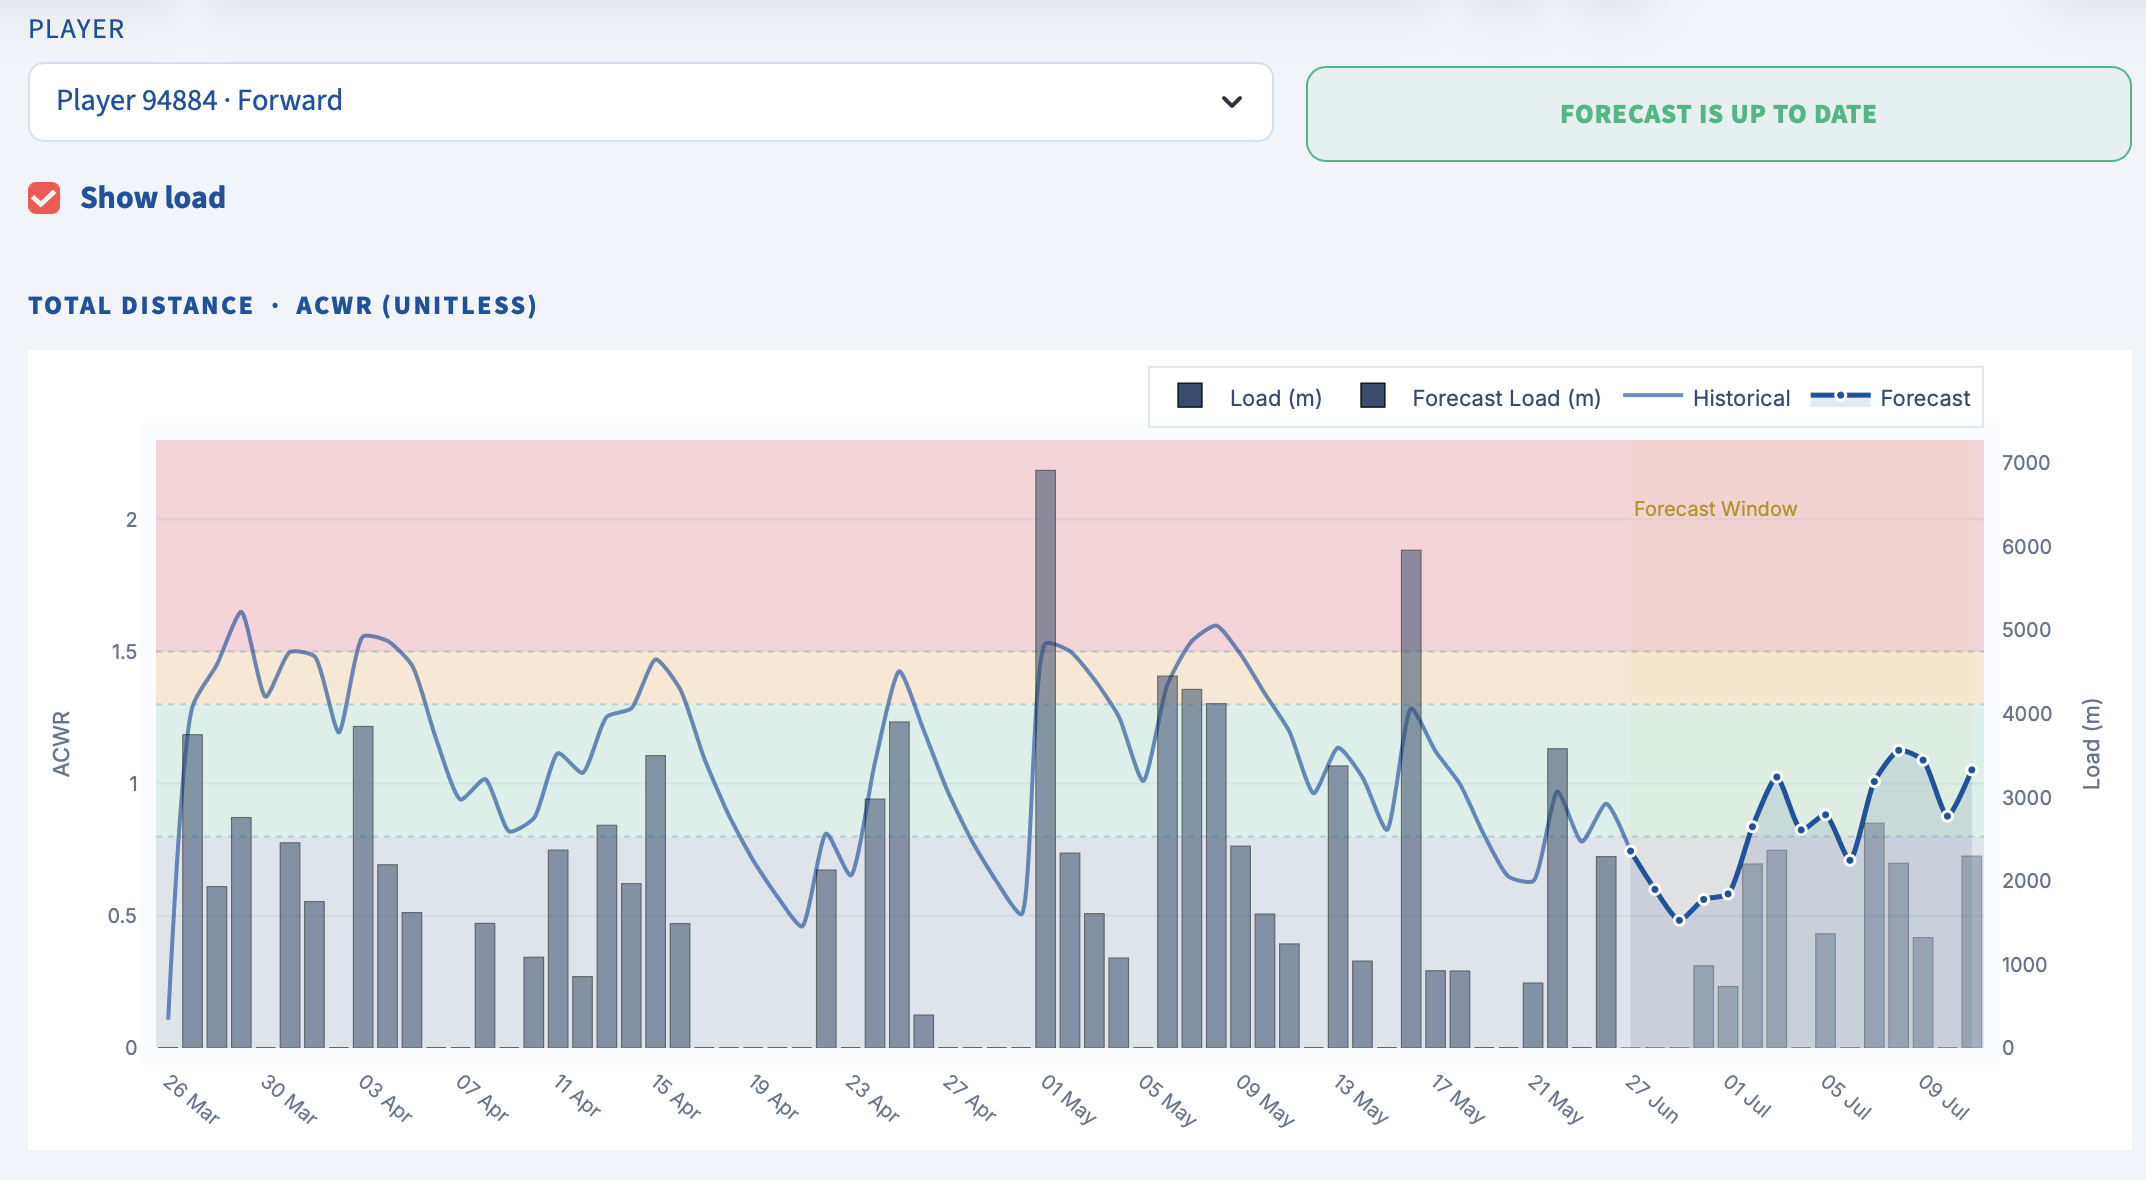
\includegraphics[width=\textwidth]{screenshots/forecast_chart.png}
\caption{Per-player forecast chart with historical ACWR, forecast ACWR, load bars, risk bands, and the forecast-window overlay.}
\label{fig:forecast-chart}
\end{figure}

The Day-15 summary table gives the final forecast ACWR for all players and all metrics. It is the fastest way to compare who remains in danger, who is merely in caution, and who ends the horizon in an optimal or undertraining zone.

\begin{figure}[H]
\centering
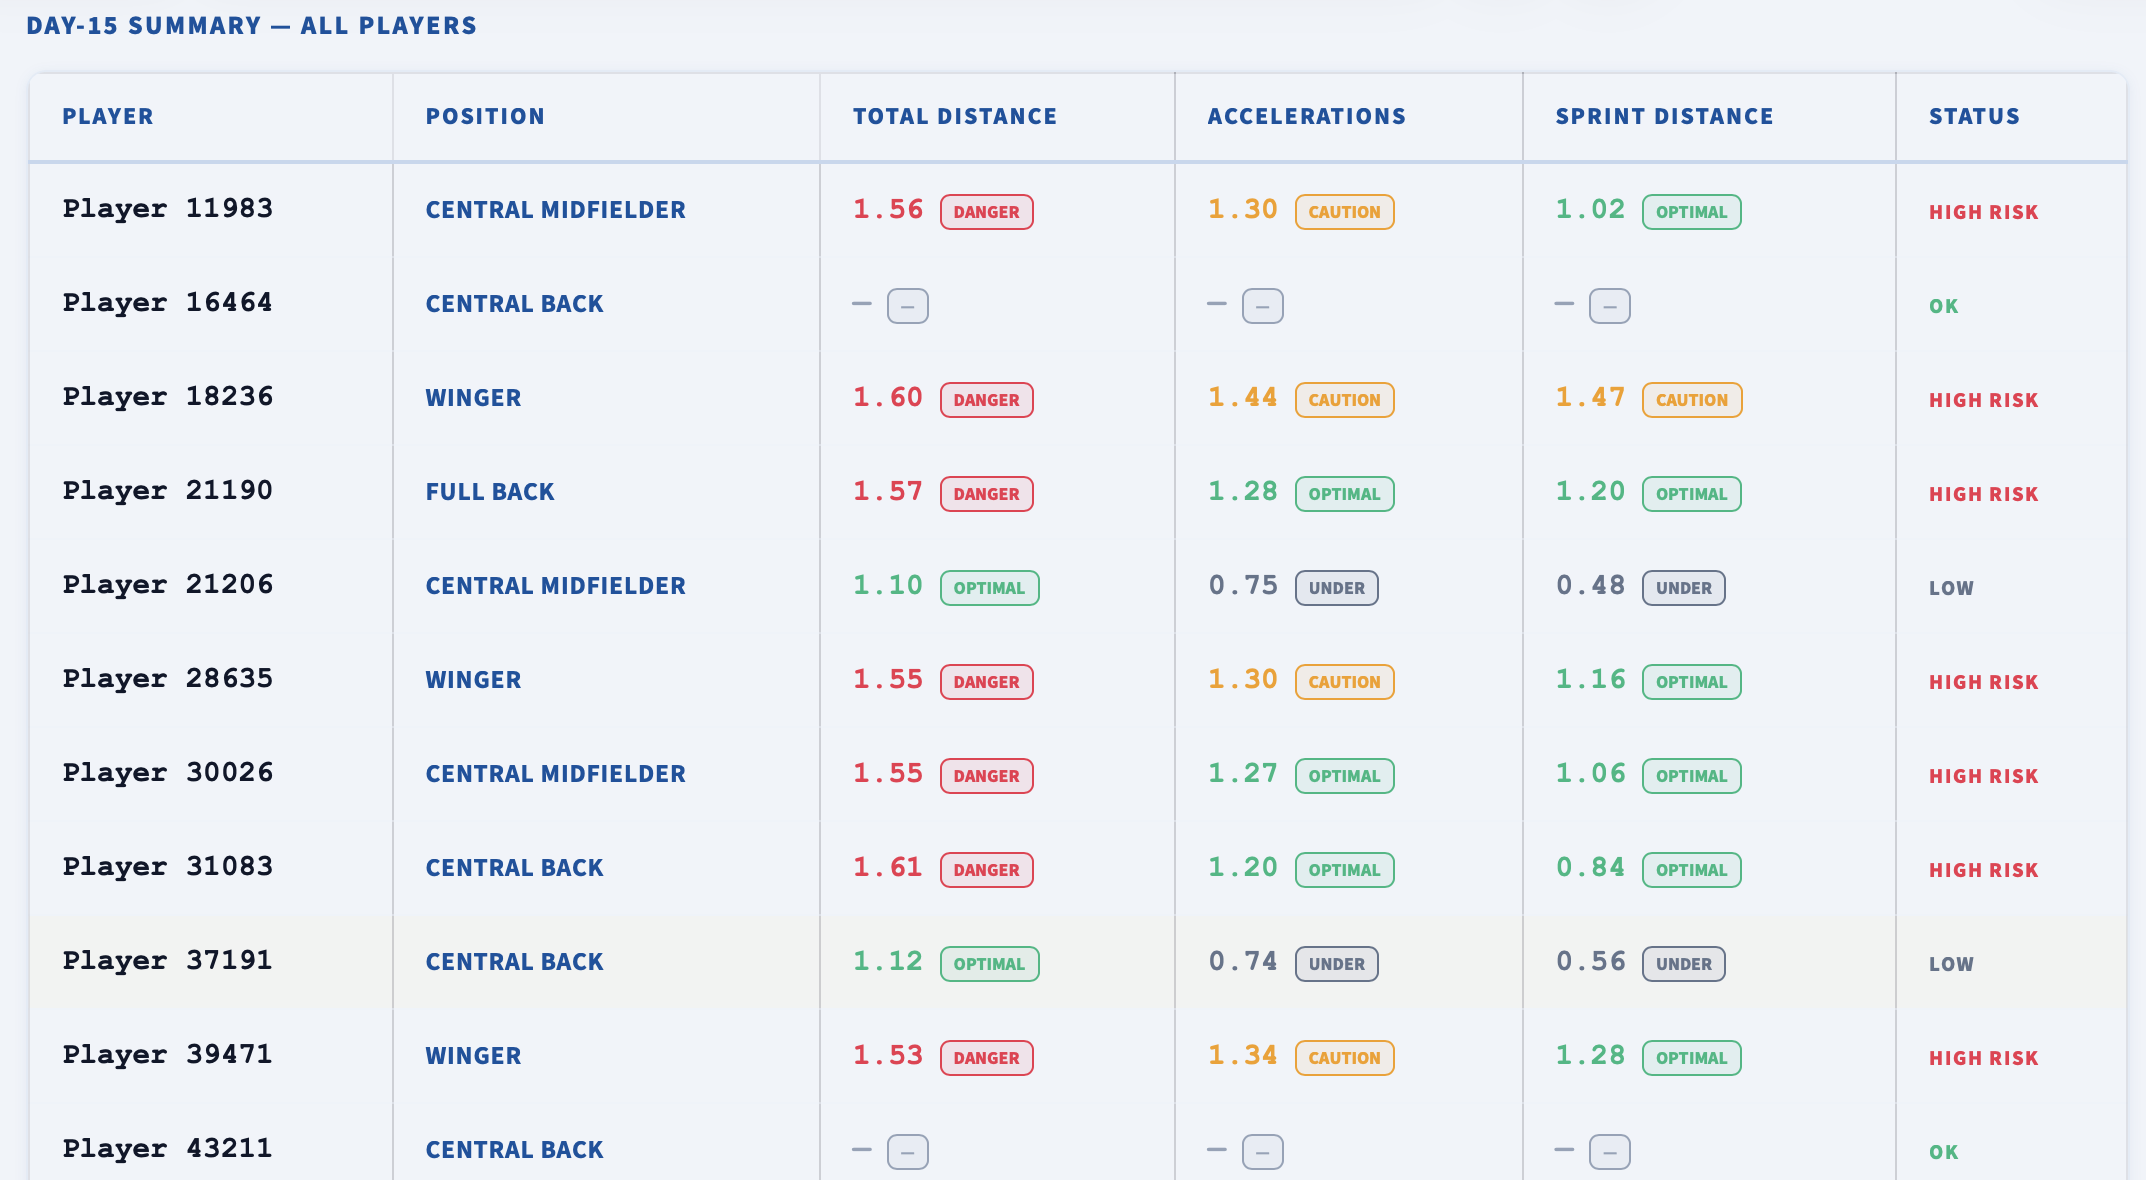
\includegraphics[width=\textwidth]{screenshots/day15_summary.png}
\caption{Day-15 summary table across all players and all monitored load metrics.}
\label{fig:day15-summary}
\end{figure}

\subsection{Player Customization}

The Player Customization page starts from the squad plan and lets coaches modify it for a single player. It is designed for players flagged as at risk after a squad forecast.

\begin{figure}[H]
\centering
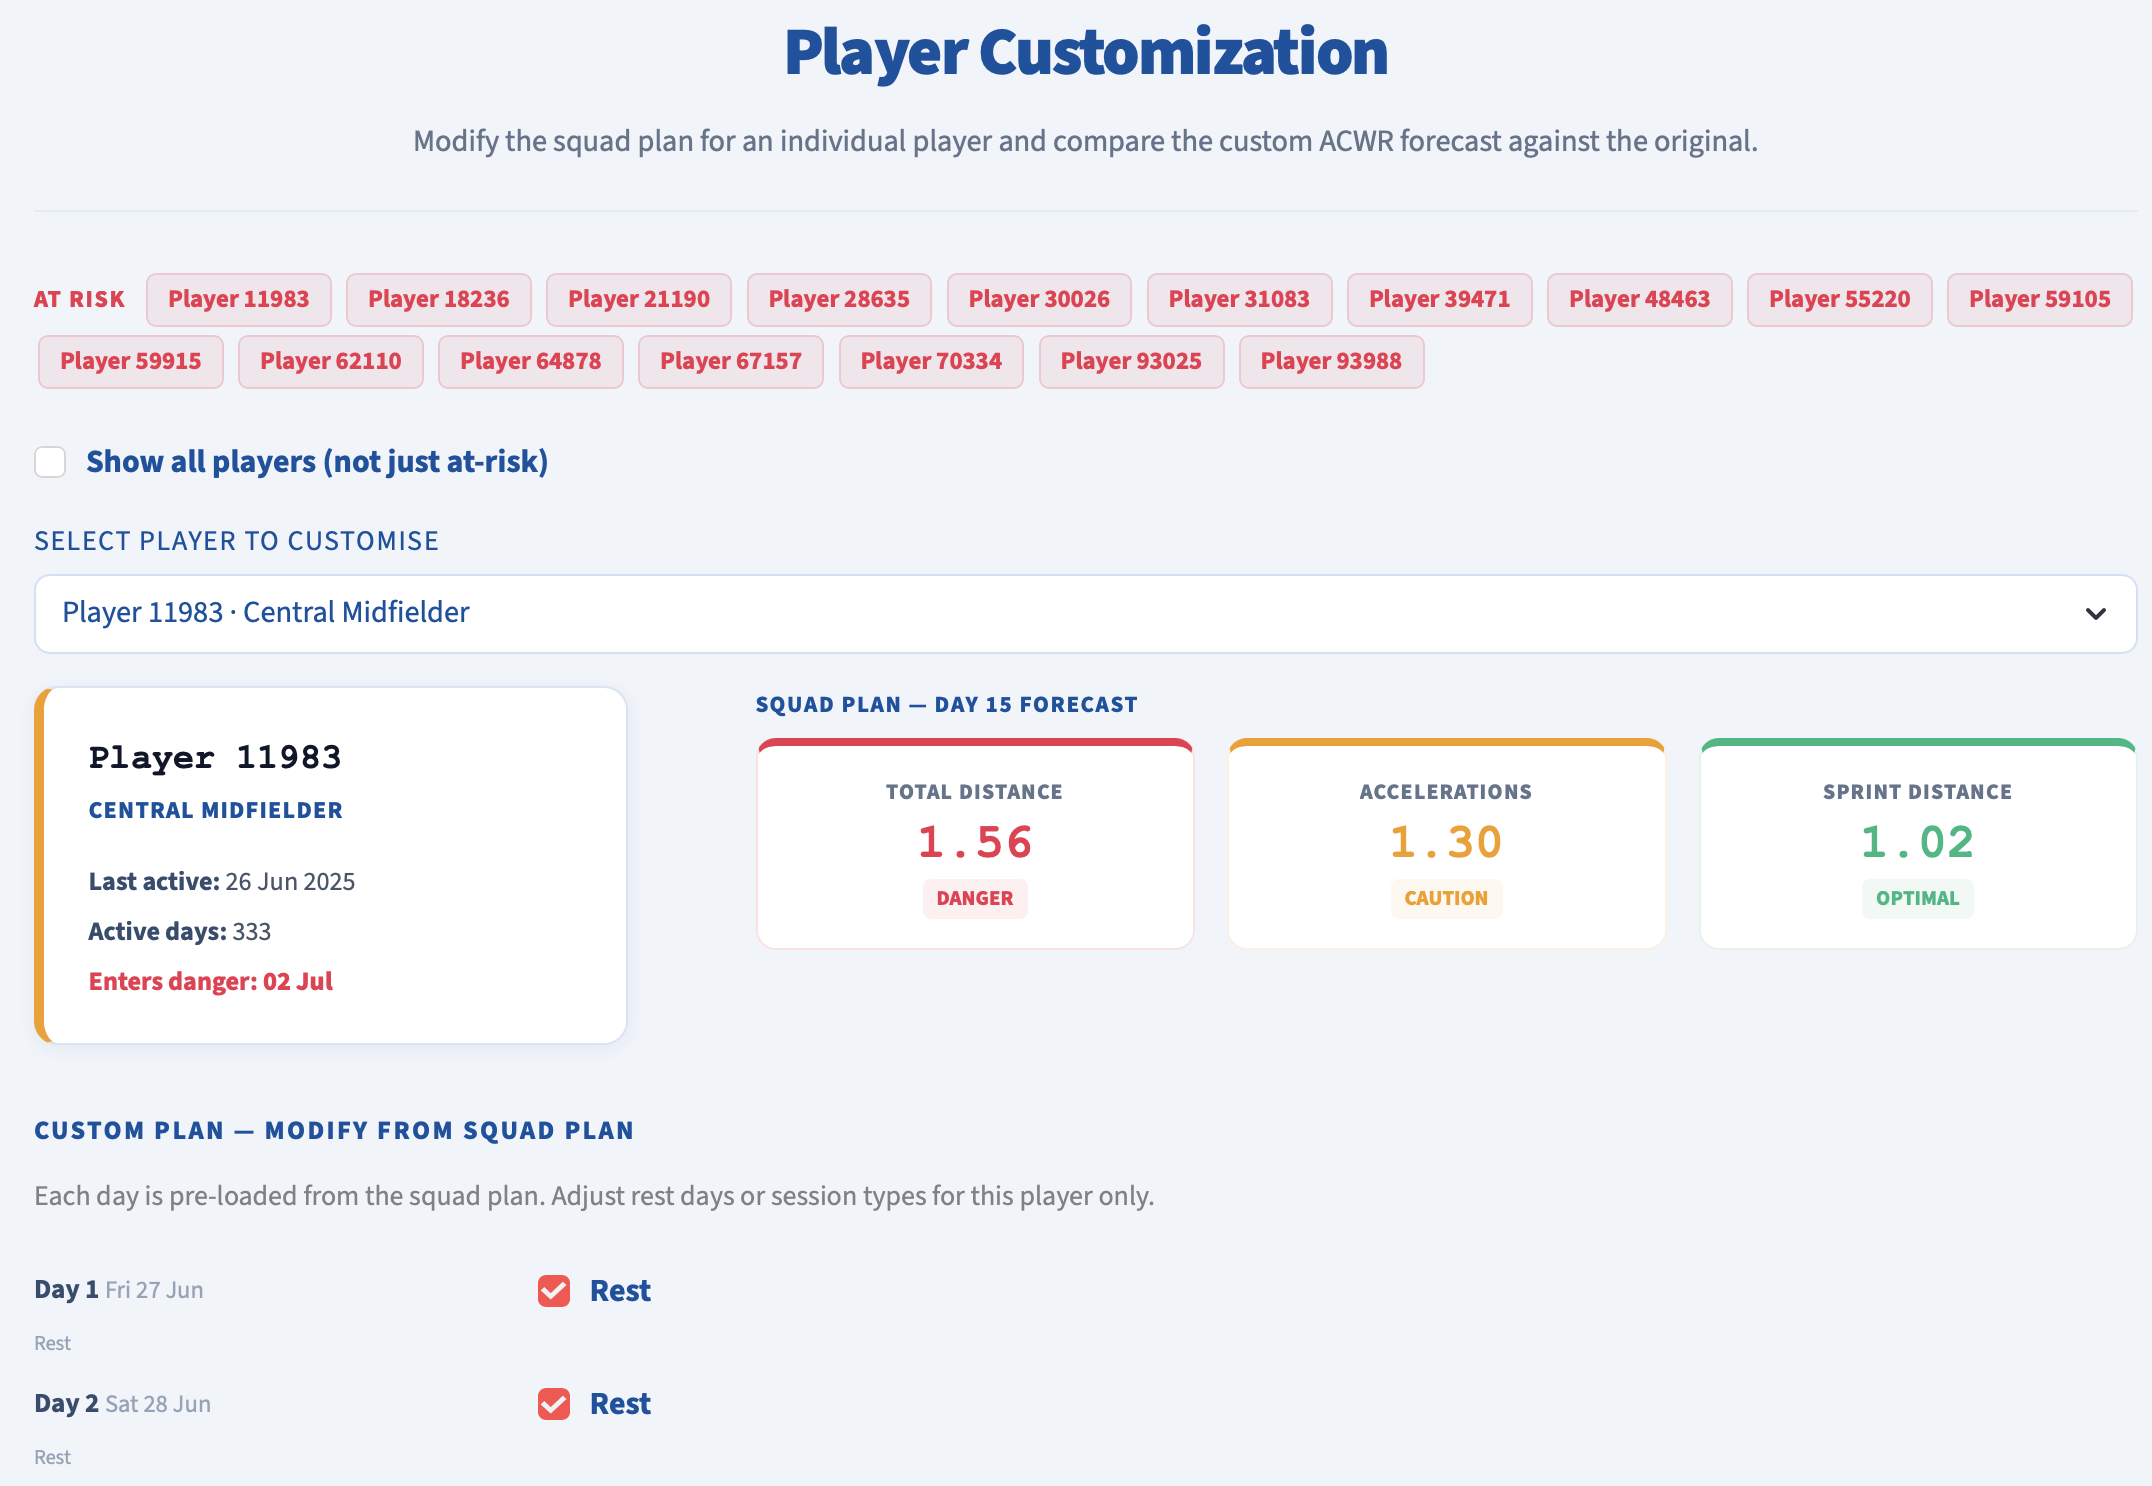
\includegraphics[width=\textwidth]{screenshots/player_customization.png}
\caption{Player-specific customization page with at-risk chips, selected player profile, squad forecast status, and editable 15-day plan rows.}
\label{fig:player-customization}
\end{figure}

Workflow:
\begin{enumerate}
  \item Run a squad forecast first on the Planning and Forecast page.
  \item Open Player Customization.
  \item Select an at-risk player, or enable the option to show all players.
  \item Modify rest days and session types for that player only.
  \item Run the player forecast.
  \item Compare squad-plan ACWR against custom-plan ACWR for each target.
\end{enumerate}

The custom plan is stored in session state and is used by the Export Plan page. Players with customized plans are marked with a custom badge in the export table.

\subsection{Export Plan}

The Export Plan page converts the effective squad plan into an A3 landscape, browser-printable HTML schedule. It uses the squad plan for most players and the customized plan for any player modified on the Player Customization page.

\begin{figure}[H]
\centering
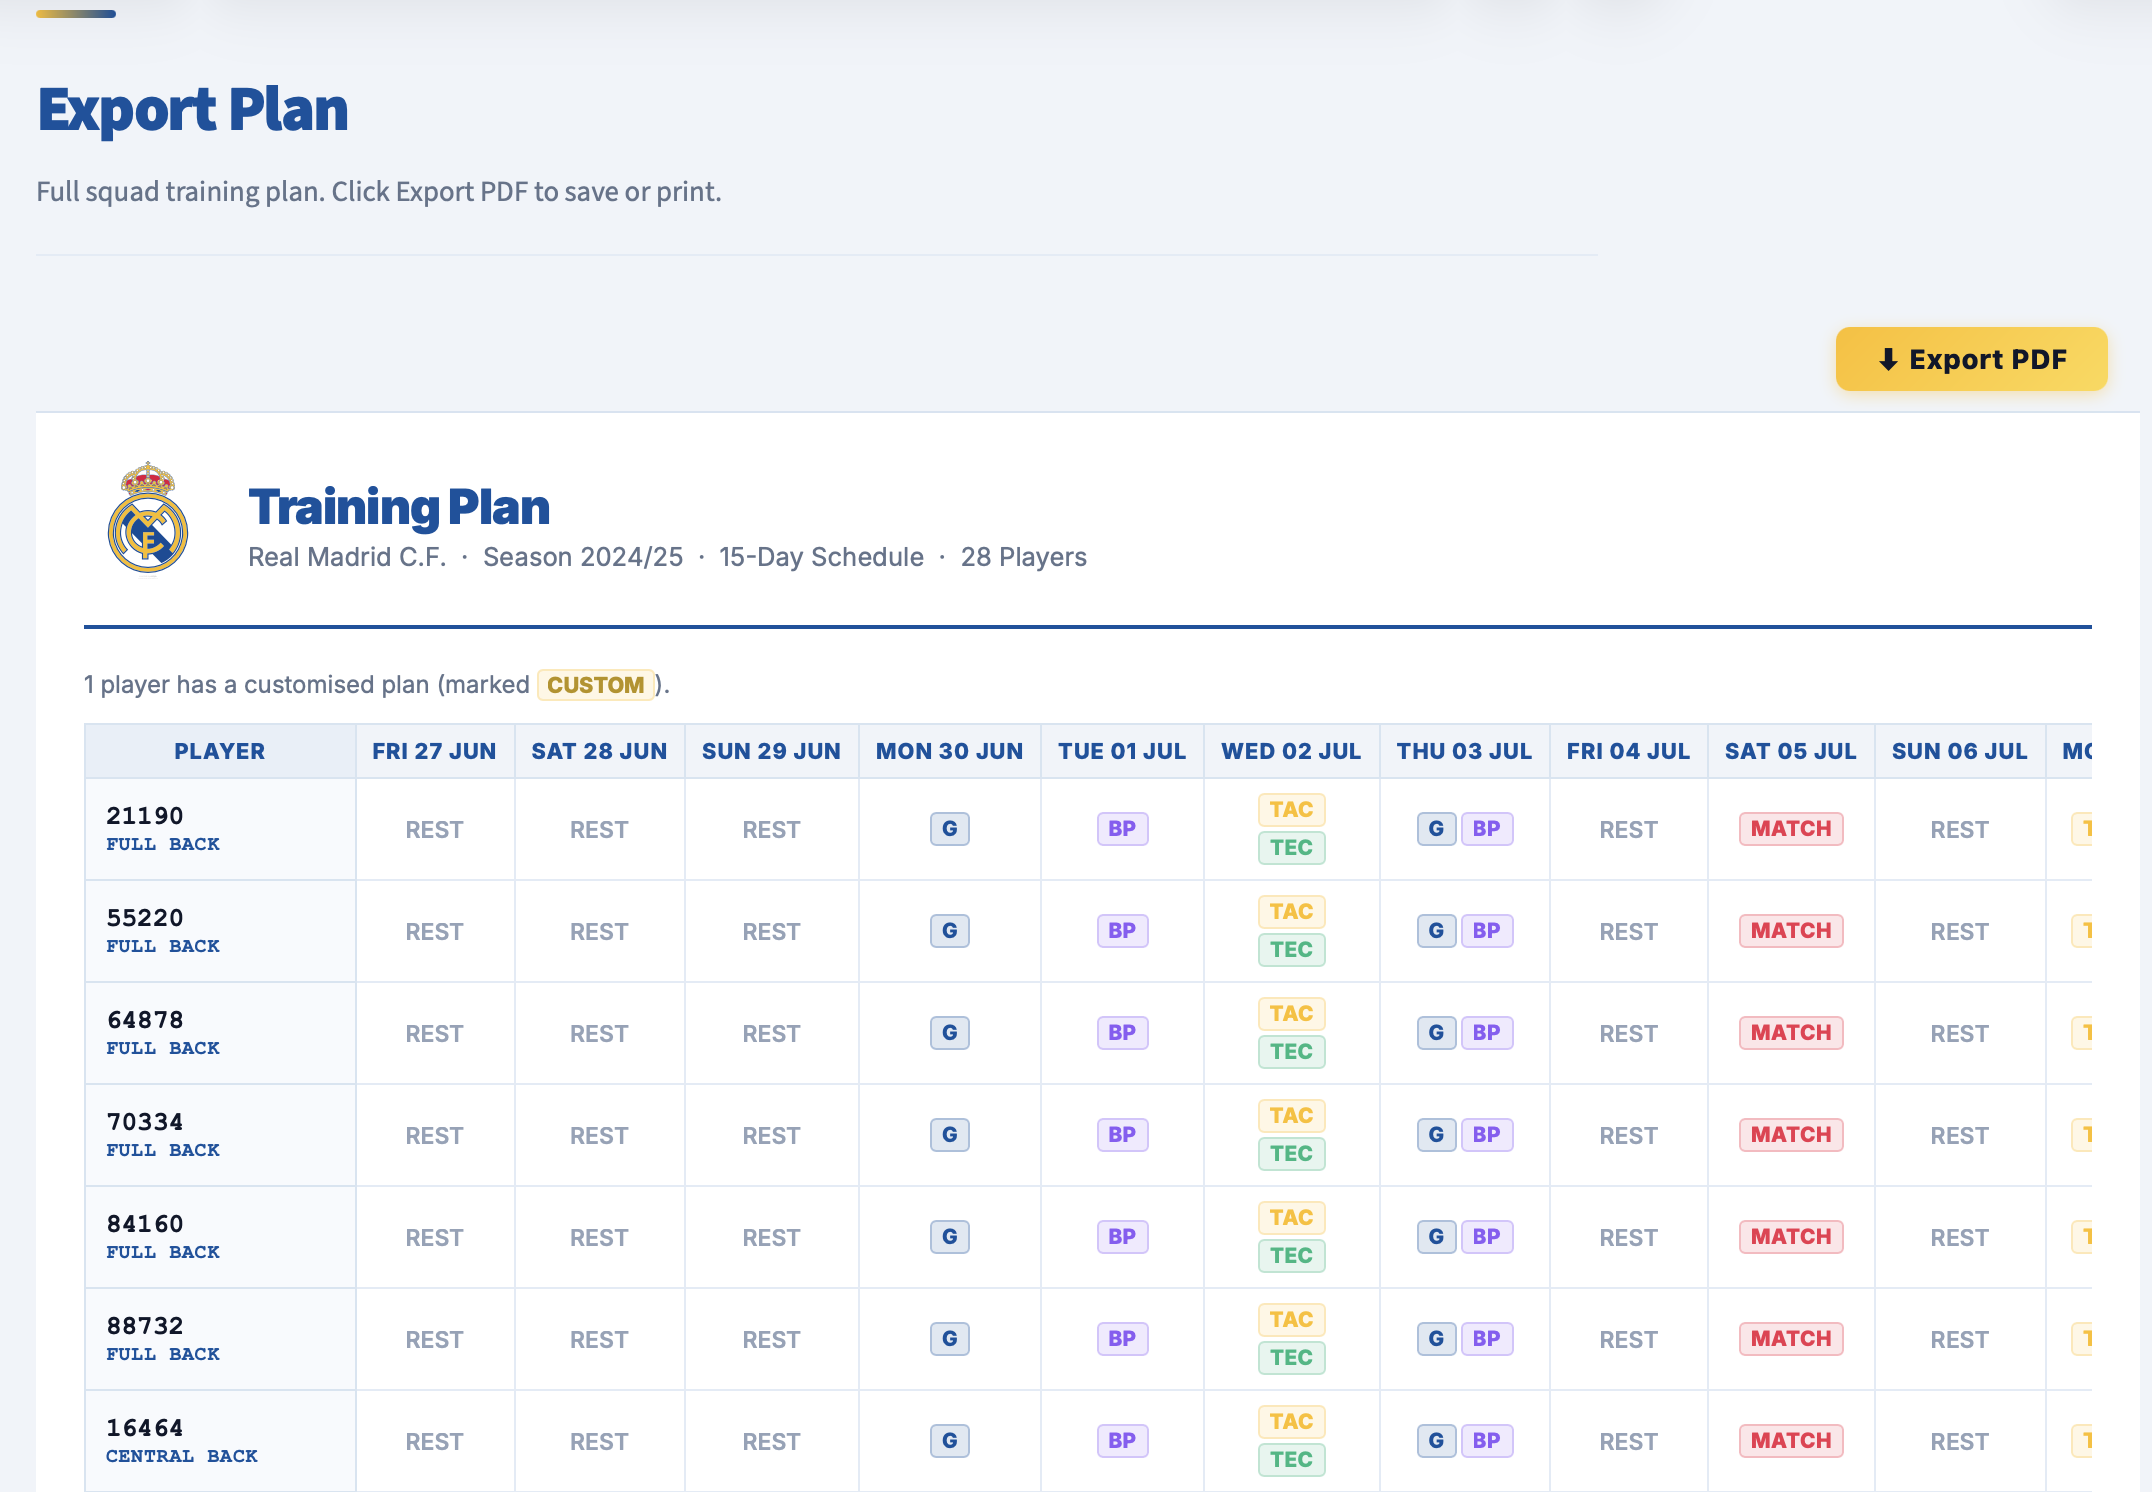
\includegraphics[width=\textwidth]{screenshots/export_plan.png}
\caption{Export page showing the full training schedule table and the export-PDF control.}
\label{fig:export-plan}
\end{figure}

Workflow:
\begin{enumerate}
  \item Run a squad forecast so the plan exists in app state.
  \item Optionally customize selected players.
  \item Open Export Plan.
  \item Review the full table by player and date.
  \item Click \textbf{Export PDF}; the browser print dialog saves or prints the plan.
\end{enumerate}

\section{Operations and Reproducibility}

\subsection{Common commands}

\begin{center}
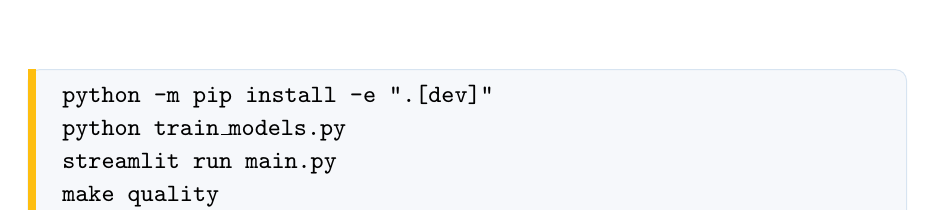
\begin{tikzpicture}
\node[
  draw=bordergray,
  fill=softgray,
  rounded corners=4pt,
  line width=0.35pt,
  inner sep=0pt
] (commandcard) {%
\begin{minipage}{0.92\textwidth}
\vspace{0.55em}
\hspace{0.9em}
\begin{minipage}{0.88\linewidth}
{\small\ttfamily
python -m pip install -e ".[dev]"\\
python train\_models.py\\
streamlit run main.py\\
make quality}
\end{minipage}
\vspace{0.55em}
\end{minipage}};
\fill[rmgold] (commandcard.north west) rectangle ([xshift=0.1cm]commandcard.south west);
\end{tikzpicture}
\end{center}

\code{python train_models.py} performs the production build: raw extraction, cleaning, outlier treatment, daily-grid creation, feature engineering, model training, and artifact writing.

\subsection{Artifact contract}

Each deployed target has exactly one artifact:

\begin{verbatim}
models/xgboost/{target}/bundle.joblib
\end{verbatim}

Each bundle must contain:
\begin{itemize}
  \item \code{model}: fitted \code{XGBRegressor};
  \item \code{scaler}: fitted \code{MinMaxScaler};
  \item \code{feature_cols}: ordered list of feature names;
  \item \code{ewma_spans}: \code{"acute": 7} and \code{"chronic": 28}.
\end{itemize}

The app validates all bundles before rendering. If a bundle is missing or malformed, the app stops and asks the operator to regenerate artifacts with \code{python train_models.py}.

\subsection{Testing and quality}

The repository includes tests for ACWR utilities, planning helpers, forecast behavior, page contracts, and artifact loading. The standard quality command is:

\begin{verbatim}
make quality
\end{verbatim}

This runs Ruff, mypy, and pytest.

\section{Assumptions and Limitations}

\begin{itemize}
  \item The data covers one season only, from July 2024 through June 2025.
  \item The model does not include wellness, session duration, RPE, medical status, or tactical role context.
  \item Rest days and data-capture gaps are indistinguishable once the daily spine is filled.
  \item ACWR is a workload proxy and should not be read as an injury probability.
  \item The risk thresholds \(0.8\), \(1.3\), and \(1.5\) are operational sport-science heuristics.
  \item The feature set is cross-sectional; future predictions do not feed into later-day feature vectors. History affects the final ACWR through the EWMA stitching step, not through the load model.
  \item Sprint distance remains the noisiest target and has the weakest held-out \(R^2\), so coaches should interpret that metric with proportionally more caution.
\end{itemize}

\section{Summary}

The project implements a two-stage workload planning system. First, XGBoost models predict daily external load from player profile and planned session composition. Second, deterministic EWMA ACWR utilities stitch predicted loads onto each player's historical daily series and classify the resulting ratio into operational risk zones. The Streamlit interface turns that pipeline into a coaching workflow: inspect current risk, plan a 15-day schedule, review forecast alerts and charts, customize plans for at-risk players, and export the final training plan.

\end{document}
